\documentclass[a4paper,12pt,titlepage]{report}

\usepackage{graphicx}
\usepackage{booktabs}
\usepackage{amsmath}
\usepackage{hyperref}
\usepackage{fullpage}
\usepackage{caption}
\usepackage{subcaption}
\usepackage{tikz}
\usepackage{tikz3d}
\usepackage{ifthen}
\usepackage[outline]{contour}
\usepackage{color}

% Grab the required TikZ libraries
\usetikzlibrary{ hexagon
               , calc
               , backgrounds
               , positioning
               , decorations.pathreplacing
               , decorations.markings
               , arrows
               , positioning
               , automata
               , shadows
               , fit
               , shapes
               , arrows
               }

% Cache TikZ figures
\usetikzlibrary{external}
\tikzexternalize[prefix=tikzcache/]

% Remove borders etc. from links added by hyperref
\hypersetup{
	colorlinks=false,
	pdfborder={0 0 0},
}

% When adding a border around some text, this is how thick it should be.
\contourlength{1.5pt}

\title{Improving the Interconnection Network of a Brain Simulator}
\author{Jonathan Heathcote}
\date{The University of Manchester}
%\date{Draft \today}

% Number subsubsections
\setcounter{secnumdepth}{3}

\begin{document}
	
	\maketitle
	
	\begin{abstract}
		
		Many attempts to understand the vast complexity of the brain centre on
		simulating models of its behaviour. Conventional super-computer topologies
		have proven poorly suited to the communication-heavy nature of neural
		simulations resulting in the development of many special-purpose systems.
		This project aims to propose a new neural simulation architecture with a
		focus on interconnection topology.
		
		Preliminary work has assessed the performance and practicality of the
		SpiNNaker neural-simulation architecture's topology. In addition, a possible
		semi-random topology is proposed to reduce the worst-case performance of the
		network.
		
		The next stages of the project will develop a interconnection network
		simulator which will be used to evaluate and compare new interconnection
		topologies. This work will eventually lead to the design of a new
		architecture.
		
	\end{abstract}
	
	\tableofcontents
	\listoffigures
	%\listoftables
	
	\chapter{Introduction}
	
	Some high-level motivation and context to sort of set the scene before going
	into what other folk have done and what I'm hoping to do.
	
	\section{Parallel Computing}
		
		The race to drive up the speed of individual processor cores ground to a
		halt in the mid 2000s leaving designers pushed to find a use for the vast
		number of transistors made available by Moore's law. In the years that
		followed we've seen multi-core processors appearing in everything from
		mobile phones to large super computers.
		
		\subsection{Programming}
			
			Hard to program parallel systems - deadlocks, locality becomes an issue --
			things can be a long way away. Cache tries to hide this but fails to
			scale. Other approaches might work (e.g. spinnaker has slow step with
			communication happening before the next step, i.e. synchronous model).
		
		\subsection{Architecture}
			
			Lots of computers must be connected together. Current styles are largely
			regular. Each offers its own advantages to different tasks. More in
			background chapter.
	
	\section{Computational Problems}
		
		Computers are faced with a wide range of problems all of which require
		different patterns of communication between the different parts of the
		program influencing the type of interconnect topology they suit.
		
		\subsection{TODO: More Examples}
		
		\subsection{Gossiping Algorithms}
			
			Generally lots of broadcast global messaging, sometimes with low
			reliability requirements.
		
		\subsection{Fluid Dynamics}
			
			Such algorithms such as heat propagation in a material. Lots of
			computation and very local, neighbour-to-neighbour communication.
		
		\subsection{Brain Simulation}
			
			% TODO: Cite overview of computational neuroscience?
			
			The brain is an extremely powerful computer about which little is
			understood. The field of computational neuroscience hopes to bring
			understanding of the computational abilities and mechanisms of the
			brain.
			
			One approach to this problem is to try and produce simulations of models
			of the brain in order to understand and study their behaviour. These
			approaches often take the form of simulated populations of neurons, one
			of the basic building-blocks of the brain. Such models typically consist
			of a set of neurons, each connected to many other neurons.  Unlike
			digital circuits where each individual component connects to only a few
			or even one other component, neurons tend to be connected to hundreds or
			thousands of other neurons.
			
			Simulations of the brain therefore present a computational challenge as
			large amounts of communication must take place between all the neurons
			in the simulated system. Various architectures have been designed to
			solve this task and a selection are presented in Chapter
			\ref{chap:background}.
			
			TODO: What is going on in brain simulators?
	
	\section{Architecture}
		
		Two major considerations when designing an architecture are the topology and
		way in which packets will be routed around the system.
		
		\subsection{Topology}
			
			Again?
		
		\subsection{Routing}
			
			Again?
		
		\subsection{Multicast}
			
			Quite simple, really.


	\chapter{Background}
	\label{chap:background}
	
	Talk about things that have been done by others in the field and try and point
	out any holes and where the pain points are. In particular, what are the
	current "big boys" doing in top500, how do neural simulators specialise this?
	What is SpiNNaker doing?
	
	\section{Simulating Brains}
		
		\label{sec:simulating-brains}
		
		% Background on brain simulation techniques.
		
		Efforts to simulate the brain ultimately focus on building an approximate
		model of the brain's behaviour. Most current brain models attempt to capture
		the way that neurons in the brain behave and connect and communicate with
		each other. Typically, the network is expressed as a graph of processing
		elements which take inputs from other neurons and perform some simple
		computation to produce an output. This type of model is known as an
		artificial neural network (ANN).
		
		\subsection{Generations of ANN}
			
			The development of ANNs can be divided up into three coarse generations,
			each increasing their level of biological realism.
			
			The first generation of ANNs, such as the McCulloch-Pitts threshold neuron
			\cite{mcculloch43}, consisted of testing if a simple, linear function of
			the neuron's inputs was above a threshold and outputting either a `high'
			or `low' value. The function used in each neuron along with the pattern of
			connectivity in the network define the behaviour of the network as a
			whole.
			
			It was realised that communication between neurons was not level-based but
			instead appeared to be based on the rate at which electrical `spikes' are
			fired by neurons to their neighbours. The second generation of ANNs seek
			to model this by representing the `firing rate' as their output as a
			continuous value \cite{maass97}. Once again, the network's behaviour is
			defined by the functions applied by each neuron and their connectivity.
			
			The third generation of ANNs extends this idea further by realising that
			the firing rate is not the only significant factor but also the timing of
			the arrival of spikes \cite{maass01}. Typically these spiking neural
			networks (SNNs) work on the principle of `leaky integrate and fire'. Here
			each spike either positively or negatively contributes to the amount of
			`charge' stored in the neuron (that is, the charge is integrated over
			time). Once the amount of charge reaches a certain threshold the neuron
			`fires' (causing a spike to be transmitted) and the amount of charge in
			the neuron returns to zero. Charge in the neuron constantly `leaks' away
			such that if the neuron doesn't receive any spikes its charge will
			eventually return to 0. This process is demonstrated in Figure
			\ref{fig:snn-example}
			
			\begin{figure}
				\center
				\input{|"python figures/snn-example.py"}
				\caption{Example behaviour of a simple leaky-intergrate-and-fire neuron}
				\label{fig:snn-example}
			\end{figure}
		
		\subsection{Computational Challenges}
			
			Simulating ANNs, and in particular SNNs, presents a number of
			computational challenges.
			
			The first issue is that real, biological neural networks can contain
			billions of neurons. An adult human, for example, has around 85 billion
			neurons \cite{herculano09}. As a result, the size of biological-scale
			networks can be extremely large requiring vast amounts of conventional
			computational resource to model. This is conventionally achieved using
			large, parallel computers.
			
			The second issue is that each neuron in the simulation may be connected to
			thousands of others. As a result of this, huge amounts of one-to-many
			communication must take place between the processing nodes simulating such
			networks. Conventional electronic circuits, and consequently conventional
			computing systems, tend to instead feature one-to-one and one-to-few
			connections as the amount of power needed to send a signal to many places
			at once can be large.
			
			Luckily most communication which occurs in the brain is highly local which
			means that spikes don't usually need to be transmitted very far. This
			means that in parallel architectures where nodes are connected via many
			independent links, sending a spike between two different neurons is
			unlikely to use the same network resources and thus the links required
			don't need to be very fast.
			
			Neurons also tend to fire at a relatively slow rate compared to electronic
			components with firing rates being measured in terms of Hertz while modern
			electronics operate at multiple Gigahertz. As a result time-division
			multiplexing can be used to use a single processing node or communication
			channel for many different neurons and spikes respectively.
	
	
	\section{Super Computers}
		
		\label{sec:super-computers}
		
		\begin{table}
			\center
			\begin{tabular}{r l r r r l l l}
				\toprule
				Rank & Name    & Pflops& Cores  & Nodes  & Topology & Interconnect          & Sources \\
				\midrule                          
				1 & Tianhe-2   & 33.86 & 3,120,000 & 16,000 & Fat-Tree & Electrical \& Optical & \cite{dongarra13} \\
				2 & Titan      & 17.59 & 560,640   & 18,688 & 3D Torus & Electrical            & \cite{bland12} \\
				3 & Sequoia    & 17.17 & 1,572,864 & 98,304 & 5D Torus & Electrical \& Optical & \cite{prickett10} \\
				4 & K Computer & 10.51 & 705,024   & 68,544 & 6D Torus & Electrical            & \cite{fujitsu11,yokokawa11} \\
				5 & Mira       &  8.59 & 786,432   & 49,152 & 5D Torus & Electrical \& Optical & \cite{prickett10} \\
				\bottomrule
			\end{tabular}
			
			\caption{Top Five `Top500' Super Computers, June 2013 \cite{meuer13}}
			\label{tab:top500}
		\end{table}
		
		The Top500 list \cite{meuer13} aims to biannually enumerate the 500 fastest
		super computers ranked by their performance on the LINPACK
		\cite{dongarraLINPAC} benchmark. The list offers an insight into the current
		state-of-the-art for high-performance computing. Table \ref{tab:top500}
		shows the top five machines in the Top500 list released in June 2013 along
		with basic details of the type of interconnection involved. In this section
		an overview is given of the architecture of these large scale machines.
		
		The LINPACK benchmark performs computations to ``analyze and solve linear
		equations and linear least-squares probles'' \cite{dongarra84} in order to
		produce a computational load representative of certain computational tasks.
		In particular it is essentially a CPU-bound problem which attempts to
		measure the peak CPU performance achievable\footnote{Where CPU Performance
		is measured in Petaflops: how many quadrillion ($10^{15}$) floating point
		operations can be performed per second.} but without any significant
		indication of the performance of the network which connects the system
		together \cite{dongarra07}.
		
		Since simulation of SNNs requires a large amount of communication combined
		with relatively small amounts of computation, this benchmark is not
		representative of the workload of such a task. Despite the shortcomings of
		the LINPACK benchmark there is unsurprisingly a high degree of correlation
		between CPU power and interconnect performance in the best Top500 machines.
		The Graph500 list is a more recent, complementary ranking which uses
		benchmarks based on graph problems \cite{murphy10}. Such problems rely on
		having efficient point-to-point communication between different parts of the
		system where each part of the graph resides. With the exception of Titan
		which was not measured, the top five Top500 computers also sit within in the
		top six places of Graph500 \cite{murphy13}. As a result, due to its maturity
		and wider scope, the Top500 list is discussed here as it is roughly
		comparable.
		
		\subsection{Anatomy of a Super-Computer}
			
			% Networks usually have a macro topology on the nodes and some local
			% topology within a node connecting many cores together.
			% Cabinets and racks
			
			Large computer systems are typically built by combining a large number of
			`processing elements' in such a way that they are able to efficiently
			communicate and work together. These processing elements come in many
			forms though the two most prevalent in the top five are:
			
			\begin{description}
				
				\item[General Purpose Processor] A conventional processor `core' as
				found in desktop and mobile computer CPUs. These flexible devices have
				historically represented the vast majority of the Top500's computing
				power.
				
				\item[Graphics Processing Unit (GPU)] A specialised processor which is
				able to efficiently perform the same operation across a large number of
				data elements simultaneously. The Titan super computer notably makes
				extensive use of GPUs \cite{bland12}.
				
			\end{description}
			
			A number of these individual cores are then combined together to create a
			single `node' in the system. Typically the cores within a node are able to
			communicate relatively cheaply while messages to remote nodes must
			traverse a slower system-wide interconnection network.
			
			Tianhe-2 makes use of Intel Ivy Bridge processors along side Intel Xeon
			Phi accelerators. The Ivy Bridge chips contain 16 general purpose
			processor cores on a single chip while the Xeon Phi contains a further
			57\footnote{The Intel Xeon Phi chip normally features 61 cores. Tianhe-2's
			Xeon Phis were taken from early production runs where manufacturing errors
			resulted in some cores being non-functional and disabled.} (somewhat
			smaller) general purpose cores \cite{dongarra13}.
			
			% TODO: Why does this section exist?
		
		\subsection{Topology}
			
			% Many cores lumped together under a single node. General topologies listed
			% in table. Inside, this depends. Xeon-Phi is a ring, GPUs are SIMD array
			% processors, some are just muti-core chips.
			
			Super computers are typically made up of a large number computing nodes
			which are connected together by some form of interconnection network.
			Typically the topology of these networks is such that local communication
			between neighbouring nodes is extremely quick and doesn't compete with
			distant nodes for communication links. The top five machines in the
			Top500 list use either `fat tree' or `torus' topologies which are
			described below.
			
			\subsubsection{Fat Tree}
			
				In a basic fat tree topology, nodes are connected to switches which in
				turn are connected to further levels of switches (Figure
				\ref{fig:fat-tree-concept}). Links higher in the switch hierarchy are
				connected via links of increasing bandwidth which avoids the bandwidth
				bottle-neck around the root node. In order for a node to communicate, it
				sends its message to its parent switch which forwards the packet through
				the tree to its destination.
				
				In practice, such as in large machines like `Tianhe-2', it is not
				possible to build a switch with the required bandwidth to build a fat
				tree. In addition, the root node acts as a single point of failure for
				the whole system. As a result, folded Clos networks are often used
				instead and have become synonymous with the fat tree topology. As shown
				in Figure \ref{fig:fat-tree-closs}, here traffic is split between the
				two top-level switches reducing the bandwidth requirement for each. In
				addition, if a top-level switch fails messages can simply be routed
				using the other switch.
				
				Fat trees give small maximum hop-counts ($O(\log{N})$ with respect to
				the number of nodes in the system) to send a message from one node to
				any other and also also allows near-by nodes to communicate in a very
				small number of hops. Unfortunately, such topologies are dependent on
				high-radix switches which can connect many nodes simultaneously.
				Tianhe-2, for example, has thirteen 576-port switches based on a custom
				router chip. The cost of such high-radix switches is typically that of
				increased latency. In the case of Tianhe-2, the latency of a message
				broadcast to all nodes in the system is around 9$\mu$s or about 19,800
				CPU\footnote{Intel Ivy Bridge CPUs running at 2.2GHz}
				cycles\cite{dongarra13}.
				
				In order to allow multiple simultaneous computation tasks to run, fat
				trees can be trivially partitioned by allocating whole sub-trees to a
				given task.
				
				\begin{figure}
					\begin{subfigure}[t]{\textwidth}
						\center
						\begin{tikzpicture}[thick, node distance=1em]
	
	\begin{scope}[every node/.style={draw,rectangle,thick},inner sep=1.0em]
		\tikzstyle{level 1}=[sibling distance=6cm,every child/.style={ultra thick},inner sep=0.8em]
		\tikzstyle{level 2}=[sibling distance=3cm,every child/.style={thick},inner sep=0.5em]
		\tikzstyle{level 3}=[sibling distance=1.5cm,every child/.style={thin},inner sep=0.1em]
		
		\node {Switch}
			child {node {Switch}
				child {node {Switch}
					child {node [circle] {Node}}
					child {node [circle] {Node}}
				}
				child {node {Switch}
					child {node [circle] {Node}}
					child {node [circle] {Node}}
				}
			}
			child {node {Switch}
				child {node {Switch}
					child {node [circle] {Node}}
					child {node [circle] {Node}}
				}
				child {node {Switch}
					child {node [circle] {Node}}
					child {node [circle] {Node}}
				}
			}
		;
	\end{scope}
	
\end{tikzpicture}

						\caption{Basic Fat Tree
						links.}
						\label{fig:fat-tree-concept}
					\end{subfigure}
					
					\vspace{1em}
					
					\begin{subfigure}[t]{\textwidth}
						\center
						\begin{tikzpicture}[thick, node distance=1em]
	
	% Level 1 switches
	\foreach \n in {0,...,1}{
		\node (level 1 \n) at (2.0cm + \n*4*1.5cm,3.0) [draw,rectangle,inner sep=0.8em] {Switch};
	}
	
	% Level 2 switches
	\foreach \n in {0,...,3}{
		\node (level 2 \n) at (0.75cm + \n*2*1.5cm,1.5) [draw,rectangle,inner sep=0.5em] {Switch};
		
		\draw [thick] (level 2 \n) to (level 1 0);
		\draw [thick] (level 2 \n) to (level 1 1);
	}
	
	% Nodes
	\foreach \n in {0,...,7}{
		\node (node \n) at (\n*1.5cm,0) [draw,circle,inner sep=0.1em] {Node};
		
		\pgfmathtruncatemacro{\switch}{\n/2}
		\draw [thin] (node \n) to (level 2 \switch);
	}
	
\end{tikzpicture}

						\caption{Folded Clos Network}
						\label{fig:fat-tree-closs}
					\end{subfigure}
					
					\caption[Fat Tree Topologies]{Fat Tree Topologies. Thicker lines
					represent higher bandwidth.}
					\label{fig:fat-tree}
				\end{figure}
			
			\subsubsection{Torus}
			
				The topology which features in all but one of the top-five, however, is
				the torus topology (also known as a $k$-ary $n$-cube). In this topology,
				nodes are arranged in a $n$-dimensional mesh. Nodes at the extreme edges
				of the mesh are connected together to form a torus.
				
				In the 2D case this can be visualised as follows. Starting with a
				regular 2D mesh (Figure \ref{fig:torus-flat}), the top- and bottom-most
				nodes being connected together to form a tube (Figure
				\ref{fig:torus-pipe}).  Then the left- and right-most nodes are
				connected together forming a torus (Figure \ref{fig:torus-3D}). Though
				hard to visualise, this process generalises to toruses of higher
				dimensions.
				
				Each node is able to communicate directly with its immediate neighbours
				in each dimension, that is above, below, left and right in this example.
				More distant nodes are able to communicate by forwarding messages via
				intermediate nodes.
				
				Because nodes in a torus only communicate directly with their
				neighbours, the routers required in each node may be of a low radix
				compared to the ones in the fat tree's switches. For an $n$-dimensional
				torus each node requires a $n+1$ router for systems containing $k^n$
				nodes where $k$ is the length of each dimension.
				
				Compared with a fat tree, however, a greater number of hops is required
				in the worst case where two nodes are distant. In a torus with $k$ nodes
				in each of $n$ dimensions the worst case path length is $\frac{kn}{2}$
				\cite{dally04}. As a result, though individual hops are less expensive,
				the time taken to broadcast a message to all nodes in a large Blue Gene/Q
				supercomputer such as Sequoia is 17.19$\mu$s compared to 9$\mu$s for the
				same operation in Tianhe-2 \cite{morozov12}.
				
				Higher dimensional toruses are also easily partitioned into a number of
				lower-dimensional toruses (with 1, 2 and 3 dimensions in the K Computer)
				or meshes to allow machines to be shared between many independent
				computing tasks \cite{yokokawa11,chen11}.
				
				\begin{figure}
					\begin{subfigure}[t]{\textwidth}
						\center
						\begin{tikzpicture}[thick,inner sep=0.1cm,3d/perspective eye={0,10,20}]
	\def\width{9}
	\def\height{9}
	
	\def\tubewidth{1}
	\def\holesize{5}
	
	\pgfmathtruncatemacro{\widthh}{\width - 1}
	\pgfmathtruncatemacro{\heightt}{\height - 1}
	
	\clip (-0.7,-0.3) rectangle (\widthh+0.7,\heightt+0.7);
	
	\foreach \lx in {0,...,\widthh}{
		\foreach \ly in {0,...,\heightt}{
			\node [fill,circle]
			      (node X\lx Y\ly) at (\lx, \ly)
			      {};
		}
	}
	
	% Draw normal links
	\foreach \x in {0,...,\widthh}{
		\foreach \y in {0,...,\heightt}{
			\pgfmathtruncatemacro{\xx}{\x + 1}
			\pgfmathtruncatemacro{\yy}{\y + 1}
			\ifthenelse{\xx < \width}{
				\draw (node X\x Y\y.center) -- (node X\xx Y\y.center);
			}{
				%\draw (node X\x Y\y.center) -- (node X0Y\y.center);
			}
			\ifthenelse{\yy < \height}{
				\draw (node X\x Y\y.center) -- (node X\x Y\yy.center);
			}{
				%\draw (node X\x Y\y.center) -- (node X\x Y0.center);
			}
		}
	}
	
	% Draw Long Links
	\foreach \x in {0,...,\widthh}{
		\draw [help lines] (node X\x Y0.center)
		            .. controls +(0.7,-2.0)
		                    and +(0.7,2.0)
		            .. (node X\x Y\heightt.center);
	}
	\foreach \y in {0,...,\heightt}{
		\draw [help lines] (node X0Y\y.center)
		            .. controls +(-2.0,0.7)
		                    and +(2.0,0.7)
		            .. (node X\widthh Y\y.center);
	}
	
\end{tikzpicture}

						\caption{Mesh (Grey lines show wrap-around connections added in a torus)}
						\label{fig:torus-flat}
					\end{subfigure}
					
					\vspace{1em}
					
					\begin{subfigure}[t]{\textwidth}
						\center
						\begin{tikzpicture}[thick,inner sep=0.1cm,3d/perspective eye={0,10,20}]
	\def\width{9}
	\def\height{9}
	
	\def\tubewidth{1}
	\def\holesize{5}
	
	\pgfmathtruncatemacro{\widthh}{\width - 1}
	\pgfmathtruncatemacro{\heightt}{\height - 1}
	
	\foreach \lx in {0,...,\widthh}{
		\foreach \ly in {0,...,\heightt}{
			\def\x{0};
			\def\y{\tubewidth};
			\def\z{0};
			
			\pgfmathsetmacro{\rotx}{(\ly*360)/\height}
			\pgfmathsetmacro{\roty}{(\lx*360)/\width}
			
			% Rotate points about x-axis depending on \ly to roll into a tube
			\pgfmathsetmacro{\xx}{\x}
			\pgfmathsetmacro{\yy}{\y*cos(\rotx) - \z*sin(\rotx)}
			\pgfmathsetmacro{\zz}{\y*sin(\rotx) + \z*cos(\rotx)}
			
			% Shift points along x-axis to make a tube
			\pgfmathsetmacro{\xxx}{\lx - (\width / 2)}
			\pgfmathsetmacro{\yyy}{\yy}
			\pgfmathsetmacro{\zzz}{\zz}
			
			\node [fill,circle]
			      (node X\lx Y\ly) at (3d cs:\xxx, \yyy, \zzz)
			      {};
		}
	}
	
	% Draw normal links
	\foreach \x in {0,...,\widthh}{
		\foreach \y in {0,...,\heightt}{
			\pgfmathtruncatemacro{\xx}{\x + 1}
			\pgfmathtruncatemacro{\yy}{\y + 1}
			\ifthenelse{\xx < \width}{
				\draw (node X\x Y\y.center) -- (node X\xx Y\y.center);
			}{
				%\draw (node X\x Y\y.center) -- (node X0Y\y.center);
			}
			\ifthenelse{\yy < \height}{
				\draw (node X\x Y\y.center) -- (node X\x Y\yy.center);
			}{
				\draw (node X\x Y\y.center) -- (node X\x Y0.center);
			}
		}
	}
	
	% Draw Long Links
	%\foreach \x in {0,...,\widthh}{
	%	\draw [red] (node X\x Y0.center)
	%	            .. controls +(0.5,-1.0)
	%	                    and +(0.5,1.0)
	%	            .. (node X\x Y\heightt.center);
	%}
	%\foreach \y in {0,...,\heightt}{
	%	\draw [red] (node X0Y\y.center)
	%	            .. controls +(-1.0,0.5)
	%	                    and +(1.0,0.5)
	%	            .. (node X\widthh Y\y.center);
	%}
	
\end{tikzpicture}

						\caption{Rolled into a Tube}
						\label{fig:torus-pipe}
					\end{subfigure}
					
					\vspace{1em}
					
					\begin{subfigure}[t]{\textwidth}
						\center
						\begin{tikzpicture}[thick,inner sep=0.1cm,3d/perspective eye={0,20,30}]
	\def\width{9}
	\def\height{9}
	
	\def\tubewidth{1}
	\def\holesize{3.5}
	
	\pgfmathtruncatemacro{\widthh}{\width - 1}
	\pgfmathtruncatemacro{\heightt}{\height - 1}
	
	\foreach \lx in {0,...,\widthh}{
		\foreach \ly in {0,...,\heightt}{
			\def\x{0};
			\def\y{\tubewidth};
			\def\z{0};
			
			\pgfmathsetmacro{\rotx}{(\ly*360)/\height}
			\pgfmathsetmacro{\roty}{(\lx*360)/\width}
			
			% Rotate points about x-axis depending on \ly to roll into a tube
			\pgfmathsetmacro{\xx}{\x}
			\pgfmathsetmacro{\yy}{\y*cos(\rotx) - \z*sin(\rotx)}
			\pgfmathsetmacro{\zz}{\y*sin(\rotx) + \z*cos(\rotx)}
			
			% Shift off axis
			\pgfmathsetmacro{\xxx}{\xx + 0}
			\pgfmathsetmacro{\yyy}{\yy + 0}
			\pgfmathsetmacro{\zzz}{\zz + \holesize}
			
			% Rotate points around y axis depending on \lx to form doughnut
			\pgfmathsetmacro{\xxxx}{(\zzz*sin(\roty)) + (\xxx*cos(\roty))}
			\pgfmathsetmacro{\yyyy}{\yyy}
			\pgfmathsetmacro{\zzzz}{(\zzz*cos(\roty)) - (\xxx*sin(\roty))}
			
			\node [fill,circle]
			      (node X\lx Y\ly) at (3d cs:\xxxx, \yyyy, \zzzz)
			      {};
		}
	}
	
	% Draw normal links
	\foreach \x in {0,...,\widthh}{
		\foreach \y in {0,...,\heightt}{
			\pgfmathtruncatemacro{\xx}{\x + 1}
			\pgfmathtruncatemacro{\yy}{\y + 1}
			\ifthenelse{\xx < \width}{
				\draw (node X\x Y\y.center) -- (node X\xx Y\y.center);
			}{
				\draw (node X\x Y\y.center) -- (node X0Y\y.center);
			}
			\ifthenelse{\yy < \height}{
				\draw (node X\x Y\y.center) -- (node X\x Y\yy.center);
			}{
				\draw (node X\x Y\y.center) -- (node X\x Y0.center);
			}
		}
	}
	
	% Draw Long Links
	%\foreach \x in {0,...,\widthh}{
	%	\draw [red] (node X\x Y0.center)
	%	            .. controls +(0.5,-1.0)
	%	                    and +(0.5,1.0)
	%	            .. (node X\x Y\heightt.center);
	%}
	%\foreach \y in {0,...,\heightt}{
	%	\draw [red] (node X0Y\y.center)
	%	            .. controls +(-1.0,0.5)
	%	                    and +(1.0,0.5)
	%	            .. (node X\widthh Y\y.center);
	%}
	
\end{tikzpicture}

						\caption{Bent into a Torus}
						\label{fig:torus-3D}
					\end{subfigure}
					
					\caption{Transforming a Mesh into a Torus}
					\label{fig:forming-a-torus}
				\end{figure}
		
		\subsection{Interconnect}
			
			%Many now using optical to transmit between cabinets. Electrical still
			%rules the waters for inter-card stuff.
			
			The physical links responsible for connecting machines together is another
			important factor in the performance achievable by a given interconnection
			system. The current state-of-the-art techniques fall into two categories:
			electrical (`high-speed serial') and, increasingly, optical transmission.
			
			Electrical transmission technologies are generally much cheaper than
			optical, especially for short distances and lower bandwidth. As a result
			connections between physically neighbouring nodes are almost universally
			connected via such links. In systems such as Blue Gene/Q and Tianhe-2
			optical links are used to connect between different cabinets in the system
			\cite{dongarra13,prickett10}. These optical links are able to carry the
			equivalent of many electrical signals over longer distances at the expense
			of more complex hardware requirements for transmitters and receivers.
			
			As is described in greater detail later in
			\S\ref{sec:wiring-up-large-spinnaker-machines} the topology of a network
			can greatly influence the difficulty of physically connecting nodes
			arranged in cabinets. Cabinets essentially map the physical nodes into an
			approximately 2D sheet. As a result, for torus networks of more than two
			dimensions, links which are physically short in higher dimensions can
			result in long wires between distant cabinets. For hierarchical networks
			such as fat trees, long wires can result from the need to connect together
			desperate parts of a system at the higher levels of the hierarchy.
			
			% TODO: What am I trying to say here?
			
			% At a very high level, these two systems operate in a similar fashion.
			% Messages are broken down into individual bits by a transmitter and then
			% sent one bit at a time across a pair of wires or a glass fibre for
			% high-speed serial and optical transmission respectively. At the receiver
			% the bits are reassembled into a complete message.
	
	\section{Hardware Neural Simulators}
		
		% Discuss various neural-simulation based approaches, e.g. neuromorphic
		% computers, Blue Brain, BrainScaleS, FPGA based things, speak to Franchesco.
		
		Current super computers are heavily focused on computation-heavy tasks as is
		apparent from the use of of hundreds of thousands of high-end processor
		cores in the Top500's top five machines. Projects such as the Blue Brain
		project \cite{markram06} attempt to make use of such computationally
		powerful machines in the simulation of relatively small ANNs of tens of
		thousands of especially realistically neurons.
		
		ANN models which use less realistic models of neuron behaviour in order to
		allow the simulation of larger networks, however, change the balance between
		computation and communication. These large networks require relatively
		little computation for each neuron but instead require vast amounts of
		communication between connected neurons. As a result, conventional super
		computer are a poor fit and alternative architectures have been developed
		for neural simulation.
		
		There are three distinct approaches being taken to designing hardware for
		neural simulation. One is to use analog electronic components for the
		entire system, another is to mix analog and digital components and a final
		approach is to use traditional digital components. These three approaches
		and their merits are described below.
		
		\subsection{Analog}
		
			Though analog computing has long been out of favour for general purpose
			computing, it has been suggested for the purpose of neural simulation as
			it is ultimately designed to match an analog system: the brain. Neural
			computing is highly fault-tolerant and is not based on the assumption
			that values will be calculated or communicated precisely. Modern digital
			computers, by contrast, have rigid requirements for the precision of
			values used in such systems and so dedicate vast amounts of hardware to
			guaranteeing such precision.
			
			A wide range of techniques for implementing the required functions in
			analog circuitry have been proposed
			\cite{graf86,holler89,agranat90,azghadi13}.  The analog circuits for
			computing functions required in neural simulations are often very simple
			and require less power than the equivalent calculations running on a
			general purpose processor \cite{misra10}. Even though the lack of
			precision yielded by analog circuits is not a problem for neural
			simulation, the lack of consistency is. The same analog circuit may have
			widely different characteristics in one part of the chip compared to
			another due to variations in the silicon wafer. In addition circuits
			must tolerate changes in temperature and voltage, a task which is
			substantially more challenging for analog circuits compared to their
			digital counterparts.
		
		\subsection{Mixed Mode}
			
			So-called `mixed mode' systems have been designed such as
			\cite{heittmann02} which combines analog computational components with
			digital memory to combine the efficient computation of analog computing
			with dense storage of digital memory. In \cite{murray91} another mixed
			mode system is given which again features analog computation of neuron
			behaviour but uses digital signals to distribute spike transmission
			allowing easier routing.
		
		\subsection{Digital}
			
			The biggest drawback of the currently proposed analog and mixed mode
			systems is that, while efficient, they are very inflexible compared to
			digital approaches which tend to be constructed from general purpose
			computing resources.
			
			The Blue Brain project, mentioned above, is also interested in simulating
			less detailed neural models. Even so, the size of such simulations is
			still limited to around 100 million neurons \cite{markram06} as the
			simulation becomes increasingly communication-bound.
			
			Others have approached this problem by developing custom, digital on-chip
			neural simulators \cite{prange93,jahnke96,schoenauer99,mehrtash03}. While
			successful in allowing relatively large numbers of neurons to be
			simulated, around 1 million in the case of \cite{mehrtash03}, these
			approaches are fundamentally restricted to only the models the designers
			originally intended. This lack of flexibility along with the increasing
			costs of designing custom silicon has pushed research away from this
			approach.
			
			FPGAs (field programmable gate arrays) are, essentially, chips which can
			be electrically programmed with custom logic circuits. They are now widely
			used in place of custom chips for performance-sensitive but highly
			specialised tasks as well as prototyping and development of conventional
			chips. Work using FPGAs to simulate neural models such as
			\cite{hellmich05} have allowed around half a million neurons with
			realistic numbers of connections between them to be simulated. Despite
			being considerably cheaper than completely custom hardware, FPGA
			development is still much slower than developing for general purpose CPUs
			and so still yields relatively inflexible systems.
	
	
	\section{SpiNNaker}
		
		\label{sec:spinnaker}
		
		% The architecture focused on by my research.
		
		The SpiNNaker project is developing a super computer architecture designed
		for running real-time simulations of large networks of SNNs. In particular,
		its designed to be `universal' in the sense that it makes few assumptions
		about the function of individual neurons \cite{furber06}. Since many
		possible neuron models exist and new ones are being produced constantly,
		this built-in flexibility escapes the fixed assumptions made by many neural
		network simulators\cite{furber07}.
		
		To achieve this flexibility SpiNNaker combines over one million
		energy-efficient, general purpose mobile phone grade CPUs with a custom
		interconnect network designed to tackle the communication bound problem of
		simulating large networks of simple neurons. The machine will be eventually
		be scaled up to support networks of around one billion ($10^9$) spiking
		neurons in real-time.
		
		Due to the machine's flexibility and novel interconnect it presents many
		opportunities for experimentation and so has been the focus of much of the
		preliminary work done so far. The rest of this section describes SpiNNaker
		highlighting areas relevant to the preliminary work and which are unique to
		the system.
		
		\subsection{Architecture}
			
			% Due to the neural networks we're using, this is the sort of topology that
			% was made. Good for sending short messages to many targets at once. Bad at
			% system stuff though, also currently very much 2D unlike the brain. Have a
			% hexagonal toroid (picture) which is nice and regular but a pain to wire up.
			
			SpiNNaker is made up of a 2D toroid\footnote{A toroid, in this context, is
			the generalisation of a torus where nodes are connected to more than four
			neighbours.} of chips where each chip connects to its six neighbouring
			chips as shown in Figure \ref{fig:spinnaker-chips}. The system can be
			flexibly extended by simply adding more chips to this arrangement. The
			size of the network is only limited by the size of address fields used by
			the routers (32 bits).
			
			Each SpiNNaker chip contains 18 low-power ARM processor cores connected
			together via a network on chip (NoC) as shown in Figure
			\ref{fig:spinnaker-chip}. Each core has a small amount of private memory
			and has access to a larger, chip-wide memory (not shown). Finally a router
			is responsible for sending and receiving messages from the six
			neighbouring chips as well as forwarding messages not destined for the
			chip.
			
			% TODO: Fix this figure as the CPUs don't really go through the NoC to the
			% router for normal use...
			
			\begin{figure}
				\center
				\begin{subfigure}[b]{0.49\textwidth}
					\center
					\begin{tikzpicture}[thick]
	
	\def\numcores{18}
	
	% Draw the cores
	\coordinate (core last);
	\foreach \n in {1,...,\numcores}{
		\pgfmathtruncatemacro{\nn}{\n-1}
		\node (core \n) [draw,rounded rectangle,minimum width=1.3cm]
		      [below=0 of core last,anchor=north west,rotate=90,inner sep=0.4ex]
		      [yshift=-0.1em]
		      {\tiny CPU \nn}
		      ;
		\draw (core \n.west) -- ++(0,-1.5);
		\coordinate (core last) at (core \n.south west);
	}
	
	% Draw the NoC cloud
	\node [cloud,draw,fill=white,cloud puffs=20,minimum width = 4cm]
	      [anchor=north,inner ysep=0.5ex,cloud ignores aspect]
	      at ([yshift=-1em]$(core 1.west)!0.5!(core 18.west)$)
	      (comms noc)
	      {Network on Chip (NoC)};
	
	% Draw the router
	\node [below=1em of comms noc]
	      [draw, rectangle, minimum width=3cm,minimum height=1.5cm]
	      (router)
	      {Router};
	
	
	% Input from NoC
	\draw [->] (comms noc.south west)
	           |- ($(router.north west)!0.15!(router.south west)$);
	
	% Output to NoC
	\draw [->] ($(router.north east)!0.15!(router.south east)$)
	           -| (comms noc.south east);
	
	% Draw inputs/outputs
	\foreach \n in {0,...,5}{
		\pgfmathsetmacro{\yperc}{0.30 + ((\n+1)/12)}
		% Inputs
		\draw [<-]
		      ($(router.north west)!\yperc!(router.south west)$)
		      -- ++(-2.2cm,0);
		% Outputs
		\draw [->]
		      ($(router.north east)!\yperc!(router.south east)$)
		      -- ++(2.2cm,0);
	}
	
	% Draw around the chip
	\newcommand*{\extractCoordinate}[3]{\path (#1); \pgfgetlastxy{#2}{#3};}
	\extractCoordinate{router.south}{\routerX}{\routerY}
	\extractCoordinate{core 1.north east}{\topLeftX}{\topLeftY}
	\extractCoordinate{core 18.south east}{\topRightX}{\topRightY}
	\draw [thin]
	      ([shift={(-1.5ex,2.0ex)}]\topLeftX,\topRightY)
	      rectangle
	      ([shift={(1.5ex,-1.5ex)}]\topRightX, \routerY);
	
\end{tikzpicture}

					\caption{SpiNNaker chip\\\color{white}.}
					\label{fig:spinnaker-chip}
				\end{subfigure}
				\begin{subfigure}[b]{0.49\textwidth}
					\center
					\begin{tikzpicture}
	
	\clip (1cm,1.25cm) rectangle +(7cm,5.25cm);
	
	\begin{scope}[hexagonXYZ,minimum size=0.25cm,inner sep=0]
		\foreach \y in {1,...,8}{
			\foreach \x in {1,...,16}{
				\node (chip \x \y) at (\x,\y) [fill,circle] {};
			}
		}
	\end{scope}
	
	\foreach \y in {2,...,7}{
		\foreach \x in {2,...,15}{
			\pgfmathtruncatemacro{\xx}{\x+1}
			\pgfmathtruncatemacro{\yy}{\y+1}
			\draw (chip \x \y) -- (chip \xx \yy);
			
			\pgfmathtruncatemacro{\xx}{\x-1}
			\pgfmathtruncatemacro{\yy}{\y-1}
			\draw (chip \x \y) -- (chip \xx \yy);
			
			\pgfmathtruncatemacro{\xx}{\x+1}
			\pgfmathtruncatemacro{\yy}{\y+0}
			\draw (chip \x \y) -- (chip \xx \yy);
			
			\pgfmathtruncatemacro{\xx}{\x-1}
			\pgfmathtruncatemacro{\yy}{\y+0}
			\draw (chip \x \y) -- (chip \xx \yy);
			
			\pgfmathtruncatemacro{\xx}{\x+0}
			\pgfmathtruncatemacro{\yy}{\y+1}
			\draw (chip \x \y) -- (chip \xx \yy);
			
			\pgfmathtruncatemacro{\xx}{\x+0}
			\pgfmathtruncatemacro{\yy}{\y-1}
			\draw (chip \x \y) -- (chip \xx \yy);
		}
	}
	
\end{tikzpicture}

					\caption{Connections (lines) between chips (dots) with wrap-around
					connections not shown}
					\label{fig:spinnaker-chips}
				\end{subfigure}
				
				\caption{Overview of the SpiNNaker architecture}
				\label{fig:spinnaker-architecture}
			\end{figure}
		
		\subsection{Routing}
			
			% Routing is done by table based router. Entries for each turn or fork in a
			% packet path. Limited number of entries. Source address based routing (TLA
			% to be requested). All routing (currently) static and offline.
			
			The on-chip router is table based meaning that routing decisions are taken
			based on pre-determined values loaded into a memory before simulations
			begin. The router operates on individual packets of data which are either
			40 or 72 bits in length. These packets are very short compared to the type
			of interconnection network commonly used in super computers. Such networks
			are typically designed to transfer larger blocks of data, possibly many
			kilobytes long, from node to node. SpiNNaker however deals with SNNs where
			only spikes need to be transmitted requiring little or no associated data.
			The system supports four different kinds of packet:
			
			\begin{description}
				
				\item[Point-to-Point (P2P)] These packets are addressed to an individual
				chip and will be passed to the core arbitrarily selected to be the `chip
				monitor'. Packets are routed using a routing table.
				
				\item[Multicast (MC)] Sent by a single core and delivered to a
				predetermined set of cores in the system. Packets are routed according
				to their source address and do not explicitly specify the destinations
				of the packet. Packets are routed using a routing table.
				
				\item[Fixed Route (FR)] Automatically routed to a predefined central
				point in the system. Used, for example, to collect diagnostic
				information back to the host machine. By not requiring an address a
				larger payload can be attached.
				
				\item[Nearest Neighbour (NN)] Routed to the immediate neighbours of a
				chip without the need for a routing table. On system start up routing
				tables have not been initialised and so NN packets are used to initially
				load the tables.
				
			\end{description}
			
			\subsubsection{Routing Scheme}
				
				% Current routing is very naive dimension order routing. Also highly
				% static and doesn't respond to network utilisation. The internet is
				% dynamic, maybe this should be too?
				
				Table based routing allows a wide array of possible routing schemes to
				be implemented conditional to two key constraints. First, the route
				taken by a packet with a particular source/destination address will
				always take the same path through the system. This is known as
				deterministic oblivious routing as the scheme is unaware of the system's
				state and cannot react to load imbalance though schemes exist which can
				improve load balance in the general case \cite{singh02}\footnote{Though
				the algorithm presented is not deterministic (it uses non-deterministic
				randomised choices) it can be approximated when the number of routes
				required is sufficiently large (as in the case of multicast routing).}.
				
				\begin{figure}
					\center
					\begin{tikzpicture}[inner sep=0]
	
	\begin{scope}[shift={(-2.0cm,3cm)},hexagonXYZ,thick]
		
		\draw [->] (0,0,0) -- (1,0,0) node [shift={(0.2,0.0,0.0)}] {$x$};
		\draw [->] (0,0,0) -- (0,1,0) node [shift={(0.0,0.2,0.0)}] {$y$};
		\draw [->] (0,0,0) -- (0,0,1) node [shift={(0.0,0.0,0.2)}] {$z$};
		
	\end{scope}
	
	\begin{scope}
		\clip (0cm,1.25cm) rectangle +(8cm,3.5cm);
		
		\begin{scope}[hexagonXYZ,minimum size=0.25cm]
			\foreach \y in {1,...,8}{
				\foreach \x in {1,...,16}{
					\node (chip \x \y) at (\x,\y) [fill,circle] {};
				}
			}
		\end{scope}
		
		\begin{scope}
			\foreach \y in {2,...,7}{
				\foreach \x in {2,...,15}{
					\pgfmathtruncatemacro{\xx}{\x+1}
					\pgfmathtruncatemacro{\yy}{\y+1}
					\draw (chip \x \y) -- (chip \xx \yy);
					
					\pgfmathtruncatemacro{\xx}{\x-1}
					\pgfmathtruncatemacro{\yy}{\y-1}
					\draw (chip \x \y) -- (chip \xx \yy);
					
					\pgfmathtruncatemacro{\xx}{\x+1}
					\pgfmathtruncatemacro{\yy}{\y+0}
					\draw (chip \x \y) -- (chip \xx \yy);
					
					\pgfmathtruncatemacro{\xx}{\x-1}
					\pgfmathtruncatemacro{\yy}{\y+0}
					\draw (chip \x \y) -- (chip \xx \yy);
					
					\pgfmathtruncatemacro{\xx}{\x+0}
					\pgfmathtruncatemacro{\yy}{\y+1}
					\draw (chip \x \y) -- (chip \xx \yy);
					
					\pgfmathtruncatemacro{\xx}{\x+0}
					\pgfmathtruncatemacro{\yy}{\y-1}
					\draw (chip \x \y) -- (chip \xx \yy);
				}
			}
		\end{scope}
	\end{scope}
	
	\node [left=0.5ex of chip 22] {\contour{white}{$S$}};
	\node [right=0.5ex of chip 95] {\contour{white}{$T$}};
	
	\draw [black,line width=3pt] (chip 22.center) -- (chip 62.center);
	\draw [black,line width=3pt] (chip 62.center) -- (chip 95.center);
	
\end{tikzpicture}


					\caption[Dimension order routing in SpiNNaker]{Dimension order routing
					in SpiNNaker showing a path from node $S$ to node $T$.}
					\label{fig:dimension-order-routing}
				\end{figure}
				
				Current versions of the routing software uses simple dimension order
				routing. Here, the three axes along which packets can travel are
				considered to be three `dimensions'\footnote{The three dimensions in
				SpiNNaker's toroid are not orthogonal as would be the case in a
				conventional torus network which is the cause of some of the slightly
				unintuitive properties of the topology.}. Packets travel along each
				dimension in turn until they can get no closer at which point they move
				onto the next dimension as shown in Figure
				\ref{fig:dimension-order-routing}. Such paths are easily computed as
				shown in \cite{nocetti02} and are minimal in length.
			
			\subsubsection{Multicast}
				
				% Not much stuff on this at the moment. I am so shit I've not read
				% anything about it anyway so that needs to change.
				
				Multicast packets allow SpiNNaker to efficiently handle the distribution
				of spikes from heavily connected nodes in the system without requiring a
				unique packet to be sent from the source to every destination. Instead a
				single packet is transmitted which is able to `fork' in order to reach
				multiple processors later in its journey.
				
				Unlike P2P packets, for which the route for every possible chip address
				(16 bits) is stored in a table, MC packets are routed based on a 32 bit
				key which uniquely identifies the neuron which fired. Exhaustively
				storing the route for every possible 32-bit key is not possible since 24
				bits are required for each entry\footnote{One bit for each of the 18
				cores and 6 external links specifying if the packet should be routed to
				that output} thus requiring a 12 gigabyte routing table.
				
				Instead of an exhaustive table, one with 1,024 entries is used. The
				router looks up the 32-bit key of MC packets and, if a matching entry
				exists, uses that entry to decide where to route the packet. If no entry
				exists in the table, the packet is forwarded to the link physically
				opposite to which it entered. As a result, the routing table only
				requires an entry when the packet changes direction or is to be
				delivered to a core.
				
				Since the route for messages with a given key won't pass through or
				change direction at most routers in the system they don't need to
				include an entry in their routing table for it. As a result this small
				size of routing table should be adequate.
				
				\begin{figure}
					\begin{subfigure}[b]{0.24\textwidth}
						\center
						\begin{tikzpicture}[inner sep=0]
	
	\begin{scope}
	\clip (0cm,1.25cm) rectangle +(3cm,3.5cm);
	
	\begin{scope}[hexagonXYZ,minimum size=0.25cm]
		\foreach \y in {1,...,8}{
			\foreach \x in {1,...,16}{
				\node (chip \x \y) at (\x,\y) [fill,circle] {};
			}
		}
	\end{scope}
	
	\begin{scope}
		\foreach \y in {2,...,7}{
			\foreach \x in {2,...,15}{
				\pgfmathtruncatemacro{\xx}{\x+1}
				\pgfmathtruncatemacro{\yy}{\y+1}
				\draw (chip \x \y) -- (chip \xx \yy);
				
				\pgfmathtruncatemacro{\xx}{\x-1}
				\pgfmathtruncatemacro{\yy}{\y-1}
				\draw (chip \x \y) -- (chip \xx \yy);
				
				\pgfmathtruncatemacro{\xx}{\x+1}
				\pgfmathtruncatemacro{\yy}{\y+0}
				\draw (chip \x \y) -- (chip \xx \yy);
				
				\pgfmathtruncatemacro{\xx}{\x-1}
				\pgfmathtruncatemacro{\yy}{\y+0}
				\draw (chip \x \y) -- (chip \xx \yy);
				
				\pgfmathtruncatemacro{\xx}{\x+0}
				\pgfmathtruncatemacro{\yy}{\y+1}
				\draw (chip \x \y) -- (chip \xx \yy);
				
				\pgfmathtruncatemacro{\xx}{\x+0}
				\pgfmathtruncatemacro{\yy}{\y-1}
				\draw (chip \x \y) -- (chip \xx \yy);
			}
		}
	\end{scope}
\end{scope}

	
	\node [left=0.5ex of chip 32] {\contour{white}{$S$}};
	\node [right=0.5ex of chip 35] {\contour{white}{$T_1$}};
	\node [right=0.5ex of chip 44] {\contour{white}{$T_2$}};
	
	\draw [black,line width=3pt]
	      (chip 32.center)
	   -- (chip 43.center)
	   -- (chip 44.center)
	      ;
	
	\draw [black,line width=3pt]
	      (chip 32.center)
	   -- (chip 35.center)
	      ;
	
\end{tikzpicture}

						\caption{}
						\label{fig:multicast-routing-a}
					\end{subfigure}
					\begin{subfigure}[b]{0.24\textwidth}
						\center
						\begin{tikzpicture}[inner sep=0]
	
	\begin{scope}
	\clip (0cm,1.25cm) rectangle +(3cm,3.5cm);
	
	\begin{scope}[hexagonXYZ,minimum size=0.25cm]
		\foreach \y in {1,...,8}{
			\foreach \x in {1,...,16}{
				\node (chip \x \y) at (\x,\y) [fill,circle] {};
			}
		}
	\end{scope}
	
	\begin{scope}
		\foreach \y in {2,...,7}{
			\foreach \x in {2,...,15}{
				\pgfmathtruncatemacro{\xx}{\x+1}
				\pgfmathtruncatemacro{\yy}{\y+1}
				\draw (chip \x \y) -- (chip \xx \yy);
				
				\pgfmathtruncatemacro{\xx}{\x-1}
				\pgfmathtruncatemacro{\yy}{\y-1}
				\draw (chip \x \y) -- (chip \xx \yy);
				
				\pgfmathtruncatemacro{\xx}{\x+1}
				\pgfmathtruncatemacro{\yy}{\y+0}
				\draw (chip \x \y) -- (chip \xx \yy);
				
				\pgfmathtruncatemacro{\xx}{\x-1}
				\pgfmathtruncatemacro{\yy}{\y+0}
				\draw (chip \x \y) -- (chip \xx \yy);
				
				\pgfmathtruncatemacro{\xx}{\x+0}
				\pgfmathtruncatemacro{\yy}{\y+1}
				\draw (chip \x \y) -- (chip \xx \yy);
				
				\pgfmathtruncatemacro{\xx}{\x+0}
				\pgfmathtruncatemacro{\yy}{\y-1}
				\draw (chip \x \y) -- (chip \xx \yy);
			}
		}
	\end{scope}
\end{scope}

	
	\node [left=0.5ex of chip 32] {\contour{white}{$S$}};
	\node [right=0.5ex of chip 35] {\contour{white}{$T_1$}};
	\node [right=0.5ex of chip 44] {\contour{white}{$T_2$}};
	
	\draw [black,line width=3pt]
	      (chip 32.center)
	   -- (chip 43.center)
	   -- (chip 44.center)
	      ;
	
	\draw [black,line width=3pt]
	      (chip 44.center)
	   -- (chip 34.center)
	   -- (chip 35.center)
	      ;
	
\end{tikzpicture}


						\caption{}
						\label{fig:multicast-routing-b}
					\end{subfigure}
					\begin{subfigure}[b]{0.24\textwidth}
						\center
						\begin{tikzpicture}[inner sep=0]
	
	\begin{scope}
	\clip (0cm,1.25cm) rectangle +(3cm,3.5cm);
	
	\begin{scope}[hexagonXYZ,minimum size=0.25cm]
		\foreach \y in {1,...,8}{
			\foreach \x in {1,...,16}{
				\node (chip \x \y) at (\x,\y) [fill,circle] {};
			}
		}
	\end{scope}
	
	\begin{scope}
		\foreach \y in {2,...,7}{
			\foreach \x in {2,...,15}{
				\pgfmathtruncatemacro{\xx}{\x+1}
				\pgfmathtruncatemacro{\yy}{\y+1}
				\draw (chip \x \y) -- (chip \xx \yy);
				
				\pgfmathtruncatemacro{\xx}{\x-1}
				\pgfmathtruncatemacro{\yy}{\y-1}
				\draw (chip \x \y) -- (chip \xx \yy);
				
				\pgfmathtruncatemacro{\xx}{\x+1}
				\pgfmathtruncatemacro{\yy}{\y+0}
				\draw (chip \x \y) -- (chip \xx \yy);
				
				\pgfmathtruncatemacro{\xx}{\x-1}
				\pgfmathtruncatemacro{\yy}{\y+0}
				\draw (chip \x \y) -- (chip \xx \yy);
				
				\pgfmathtruncatemacro{\xx}{\x+0}
				\pgfmathtruncatemacro{\yy}{\y+1}
				\draw (chip \x \y) -- (chip \xx \yy);
				
				\pgfmathtruncatemacro{\xx}{\x+0}
				\pgfmathtruncatemacro{\yy}{\y-1}
				\draw (chip \x \y) -- (chip \xx \yy);
			}
		}
	\end{scope}
\end{scope}

	
	\node [left=0.5ex of chip 32] {\contour{white}{$S$}};
	\node [right=0.5ex of chip 35] {\contour{white}{$T_1$}};
	\node [right=0.5ex of chip 44] {\contour{white}{$T_2$}};
	
	\draw [black,line width=3pt]
	      (chip 34.center)
	   -- (chip 44.center)
	      ;
	
	\draw [black,line width=3pt]
	      (chip 32.center)
	   -- (chip 35.center)
	      ;
	
\end{tikzpicture}


						\caption{}
						\label{fig:multicast-routing-c}
					\end{subfigure}
					\begin{subfigure}[b]{0.24\textwidth}
						\center
						\begin{tikzpicture}[inner sep=0]
	
	\begin{scope}
	\clip (0cm,1.25cm) rectangle +(3cm,3.5cm);
	
	\begin{scope}[hexagonXYZ,minimum size=0.25cm]
		\foreach \y in {1,...,8}{
			\foreach \x in {1,...,16}{
				\node (chip \x \y) at (\x,\y) [fill,circle] {};
			}
		}
	\end{scope}
	
	\begin{scope}
		\foreach \y in {2,...,7}{
			\foreach \x in {2,...,15}{
				\pgfmathtruncatemacro{\xx}{\x+1}
				\pgfmathtruncatemacro{\yy}{\y+1}
				\draw (chip \x \y) -- (chip \xx \yy);
				
				\pgfmathtruncatemacro{\xx}{\x-1}
				\pgfmathtruncatemacro{\yy}{\y-1}
				\draw (chip \x \y) -- (chip \xx \yy);
				
				\pgfmathtruncatemacro{\xx}{\x+1}
				\pgfmathtruncatemacro{\yy}{\y+0}
				\draw (chip \x \y) -- (chip \xx \yy);
				
				\pgfmathtruncatemacro{\xx}{\x-1}
				\pgfmathtruncatemacro{\yy}{\y+0}
				\draw (chip \x \y) -- (chip \xx \yy);
				
				\pgfmathtruncatemacro{\xx}{\x+0}
				\pgfmathtruncatemacro{\yy}{\y+1}
				\draw (chip \x \y) -- (chip \xx \yy);
				
				\pgfmathtruncatemacro{\xx}{\x+0}
				\pgfmathtruncatemacro{\yy}{\y-1}
				\draw (chip \x \y) -- (chip \xx \yy);
			}
		}
	\end{scope}
\end{scope}

	
	\node [left=0.5ex of chip 32] {\contour{white}{$S$}};
	\node [right=0.5ex of chip 35] {\contour{white}{$T_1$}};
	\node [right=0.5ex of chip 44] {\contour{white}{$T_2$}};
	
	\draw [black,line width=3pt]
	      (chip 33.center)
	   -- (chip 44.center)
	      ;
	
	\draw [black,line width=3pt]
	      (chip 32.center)
	   -- (chip 35.center)
	      ;
	
\end{tikzpicture}


						\caption{}
						\label{fig:multicast-routing-d}
					\end{subfigure}
					\caption{Possible multicast routings from $S$ to $T_1$ and $T_2$}
					\label{fig:multicast-routing}
				\end{figure}
				
				In multicast routing, the choice of where a route should fork can have a
				great impact on both system load, packet latency and routing table entry
				usage. Figure \ref{fig:multicast-routing} shows several examples of
				valid multicast routings which fork at different points, each with
				differing trade-offs. Figures (b) - (d) are all optimal in the total
				number of `hops' required while (a), (c) and (d) are optimal in the
				number of routing entries required.
				
				As well as guaranteeing no routing table requires more than 1,024
				entries the routing scheme chosen must attempt to ensure an even
				load-balance by avoiding over-using certain links. Various heuristic
				approaches based on extensions to Lee's algorithm have been proposed for
				future versions of the routing software\cite{davidson13}.
			
			\subsubsection{Emergency Routing}
				
				If a packet's intended route is blocked, for example due to a bad link,
				`emergency routing' via an adjacent chip can optionally be attempted as
				shown in Figure \ref{fig:emergency-routing}. This novel approach allows
				the system to automatically recover from certain link failures without
				immediate manual intervention.
				
				\begin{figure}
					\center
					\begin{tikzpicture}[inner sep=0]
	
	\clip (2cm,1.25cm) rectangle +(3cm,3.5cm);
	
	\begin{scope}[hexagonXYZ,minimum size=0.25cm,inner sep=0]
		\foreach \y in {1,...,8}{
			\foreach \x in {1,...,16}{
				\node (chip \x \y) at (\x,\y) [fill,circle] {};
			}
		}
	\end{scope}
	
	\begin{scope}
		\foreach \y in {2,...,7}{
			\foreach \x in {2,...,15}{
				\pgfmathtruncatemacro{\xx}{\x+1}
				\pgfmathtruncatemacro{\yy}{\y+1}
				\draw (chip \x \y) -- (chip \xx \yy);
				
				\pgfmathtruncatemacro{\xx}{\x-1}
				\pgfmathtruncatemacro{\yy}{\y-1}
				\draw (chip \x \y) -- (chip \xx \yy);
				
				\pgfmathtruncatemacro{\xx}{\x+1}
				\pgfmathtruncatemacro{\yy}{\y+0}
				\draw (chip \x \y) -- (chip \xx \yy);
				
				\pgfmathtruncatemacro{\xx}{\x-1}
				\pgfmathtruncatemacro{\yy}{\y+0}
				\draw (chip \x \y) -- (chip \xx \yy);
				
				\pgfmathtruncatemacro{\xx}{\x+0}
				\pgfmathtruncatemacro{\yy}{\y+1}
				\draw (chip \x \y) -- (chip \xx \yy);
				
				\pgfmathtruncatemacro{\xx}{\x+0}
				\pgfmathtruncatemacro{\yy}{\y-1}
				\draw (chip \x \y) -- (chip \xx \yy);
			}
		}
	\end{scope}
	
	\node [below right=0.5ex of chip 53] {\contour{white}{$S$}};
	\node [below right=0.5ex of chip 64] {\contour{white}{$T$}};
	
	\draw [white,ultra thick=3pt] (chip 53) -- (chip 64);
	\draw [style=help lines] (chip 53) -- coordinate (badlink) (chip 64);
	
	\draw [red,thick]
	      ([shift={(-0.7ex,-0.7ex)}]badlink)
	   -- ([shift={(+0.7ex,+0.7ex)}]badlink)
	      ([shift={(-0.7ex,+0.7ex)}]badlink)
	   -- ([shift={(+0.7ex,-0.7ex)}]badlink);
	
	\draw [black,line width=3pt] (chip 53.center) -- (chip 54.center);
	\draw [black,line width=3pt] (chip 54.center) -- (chip 64.center);
	
\end{tikzpicture}


					\caption{Emergency route from $S$ to $T$ when the normal route is
					unavailable.}
					\label{fig:emergency-routing}
				\end{figure}
			
		
		\subsection{Hardware Abstractions}
			
			% SpiNNaker is made up of 18 core chips on 48-chip boards in 12 card racks
			% in 5-rack cabinets in a 10 cabinet system. Woah.
			
			The largest SpiNNaker system will contain 1,036,800 cores in 57,600 chips.
			These chips are split up into 1,200 circuit boards of 48 chips each as
			shown in Figure \ref{fig:spinn4labelled}.
			
			\begin{figure}
				\center
				\begin{tikzpicture}[thick]
	
	\node[anchor=south west,inner sep=0] at (0,0) (image)
		{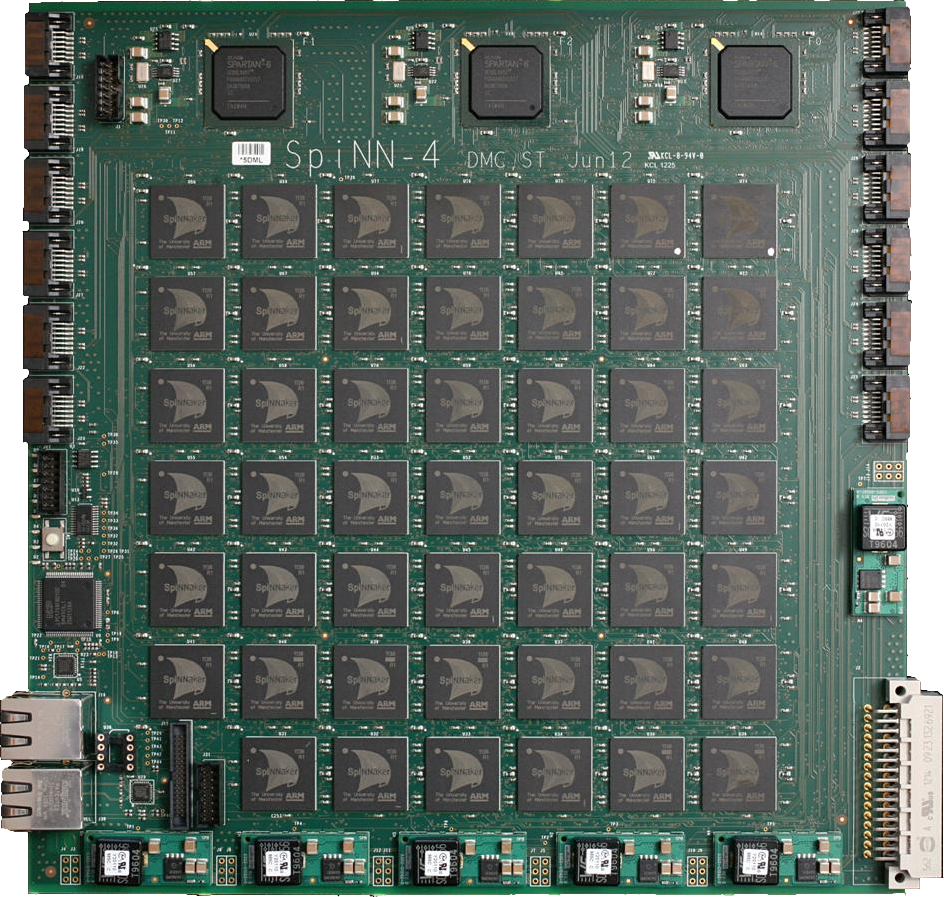
\includegraphics[width=0.5\textwidth]{figures/spinn4.png}};
	
	\begin{scope}[x={(image.south east)},y={(image.north west)}]
		%% Help with drawing
		%\draw[help lines,xstep=.1,ystep=.1] (0,0) grid (1,1);
		%\foreach \x in {0,1,...,9} { \node [anchor=north] at (\x/10,0) {0.\x}; }
		%\foreach \y in {0,1,...,9} { \node [anchor=east] at (0,\y/10) {0.\y}; }
		
		\draw [decorate,decoration={brace,raise=1ex,amplitude=1ex}]
		      (0.02,0.5) -- coordinate (left-label) (0.02,1.0);
		\node [left=1em of left-label,text width=3.5cm,align=center]
		      {High-Speed Links\\(Board-to-Board)};
		
		\draw [decorate,decoration={brace,raise=1ex,amplitude=1ex}]
		      (0.97,1.0) -- coordinate (right-label) (0.97,0.5);
		\node [right=1em of right-label,text width=3.5cm,align=center]
		      {High-Speed Links\\(Other I/O)};
		
		\draw [decorate,decoration={brace,raise=1ex,amplitude=1ex}]
		      (1.0,0.23) -- coordinate (power-label) (1.0,0.02);
		\node [right=1em of power-label] {Power Connector};
		
		\draw [decorate,decoration={brace,raise=1ex,amplitude=1ex}]
		      (0.0,0.08) -- coordinate (eth-label) (0.0,0.22);
		\node [left=1em of eth-label] {Ethernet};
	\end{scope}
	
\end{tikzpicture}

				\caption{48-chip SpiNNaker Circuit Board}
				\label{fig:spinn4labelled}
			\end{figure}
			
			Each board is equipped with a number of high-speed links, six of which are
			used to connect the board's chips them to their neighbours on other
			boards. The other six links are reserved for connecting other I/O such as
			sensors, such as the silicon retina, and robotic platforms
			\cite{davies10}. An Ethernet connection is also present to provide a
			simple, low-bandwidth link to an external host system.
			
			\begin{figure}
				\center
				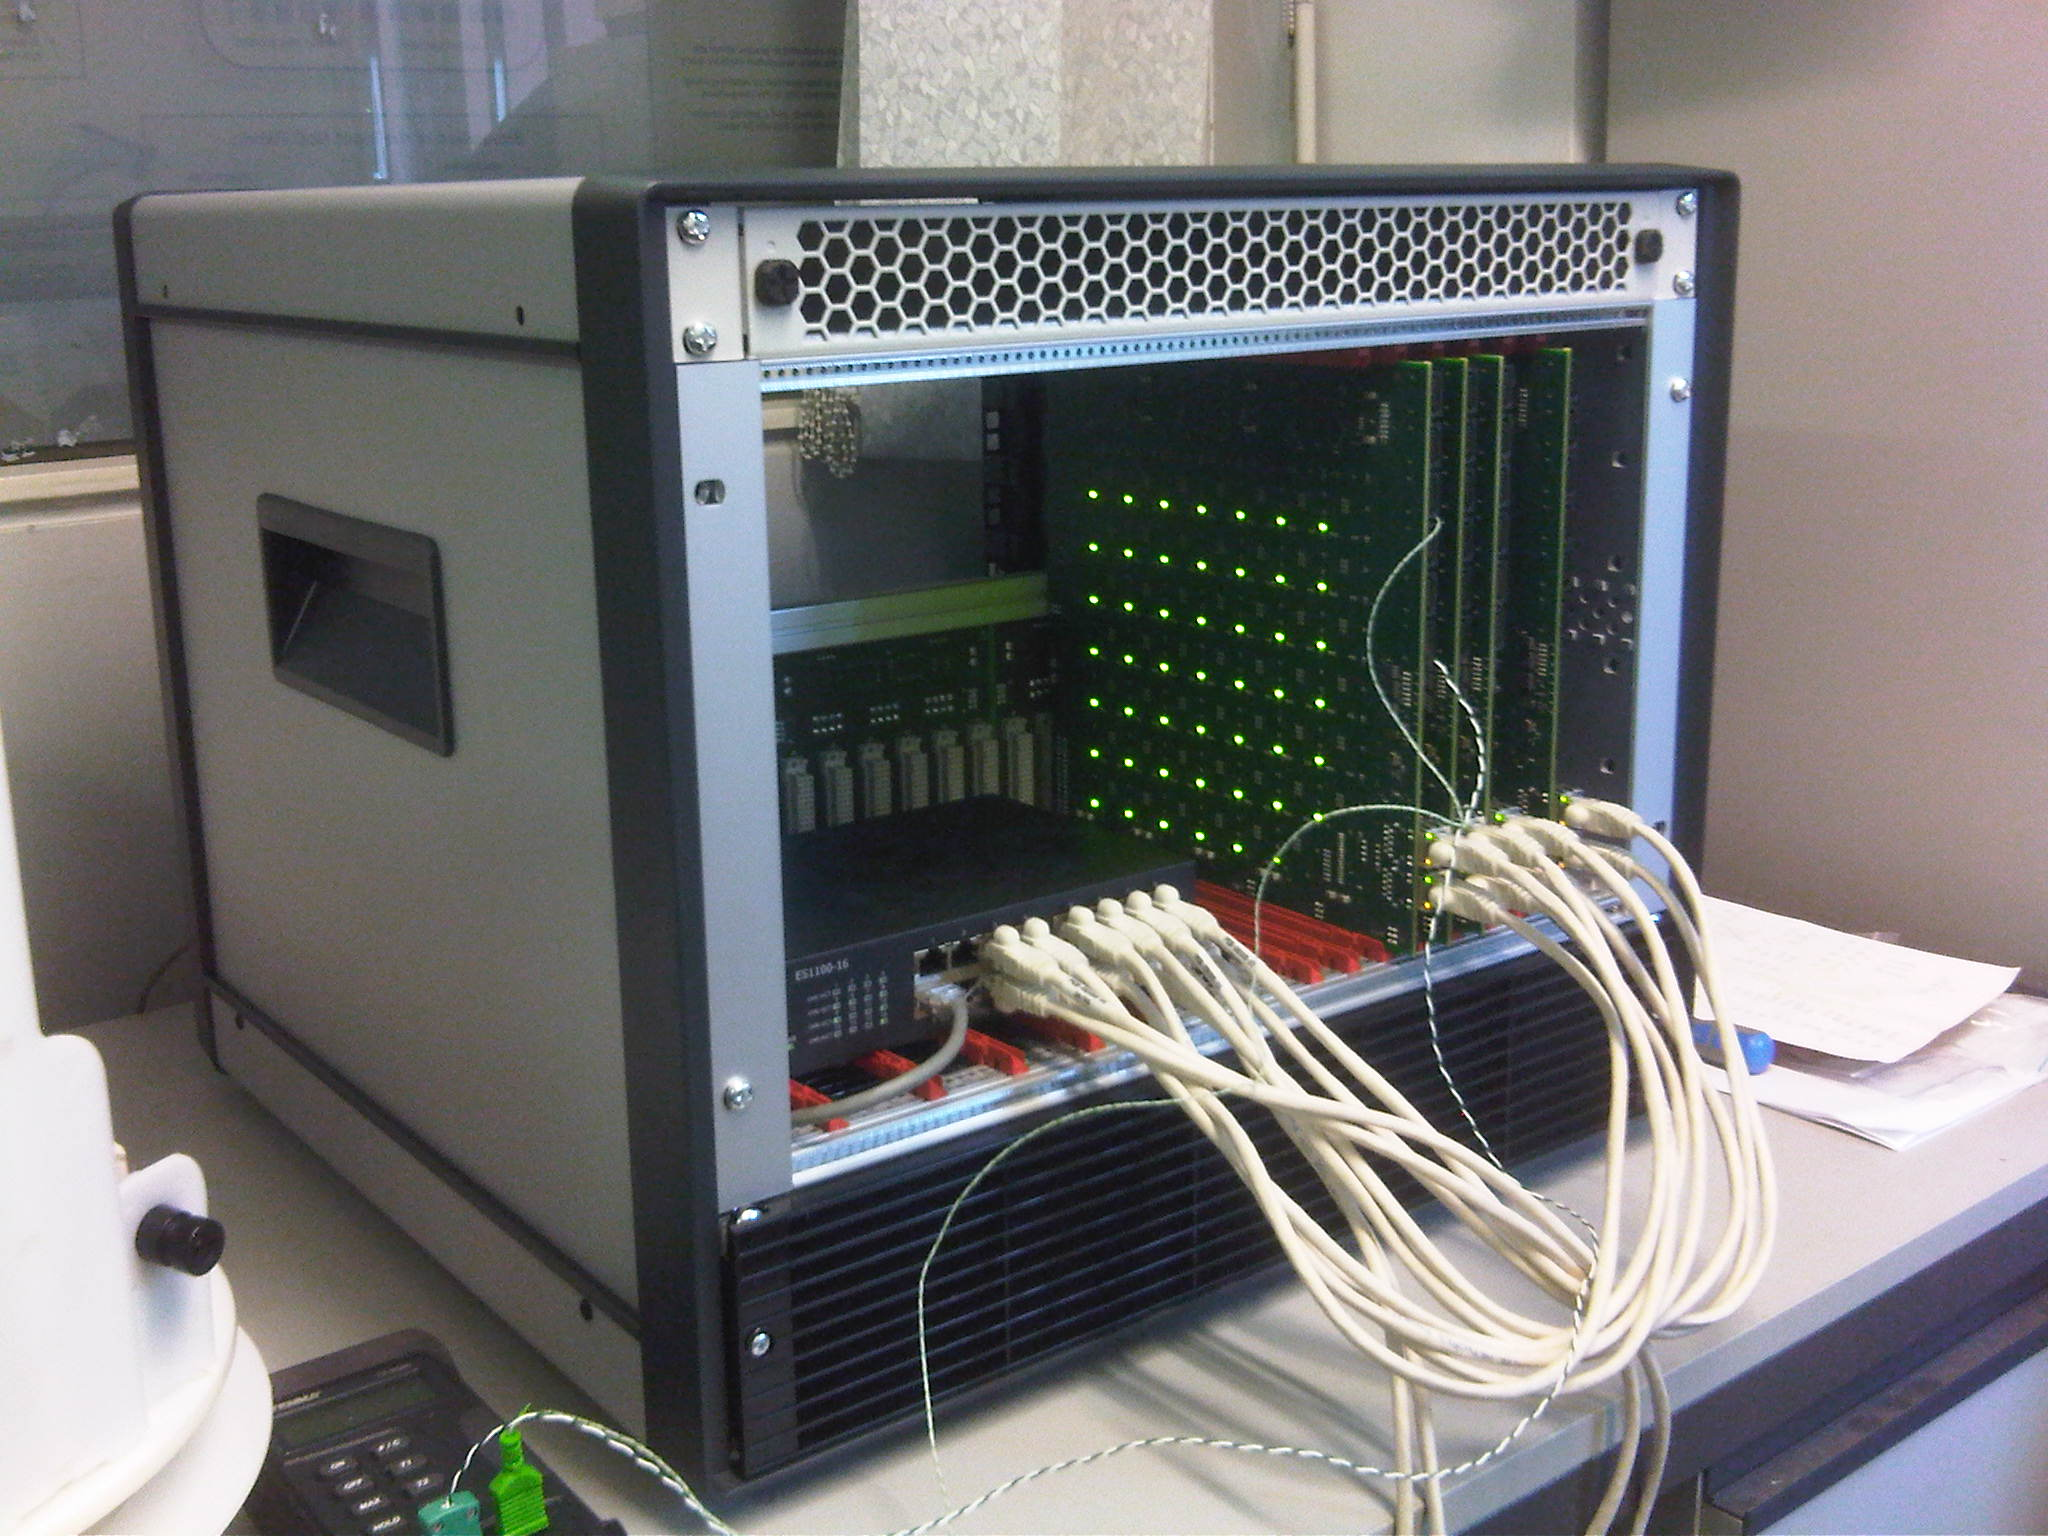
\includegraphics[width=0.5\textwidth]{figures/spiNNaker103.jpg}
				\caption{A partially populated rack of SpiNNaker boards}
				\label{fig:spiNNaker103}
			\end{figure}
			
			Twenty-four boards are then placed in racks such as in Figure
			\ref{fig:spiNNaker103} which are in turn placed, five-high, into ten
			cabinets. Further details of this arrangement are given later in
			\S\ref{sec:wiring-up-large-spinnaker-machines} where preliminary work on
			wiring schemes for the machine is described.
		
		\subsection{Connecting Boards Together}
			
			% Describe what the edge links have.  Boards are connected together via high
			% speed serial links. 8 links per board. First gen had two spare
			% connections, new one has ring and one spare. What can the spares be used
			% for?
			
			% TODO: Reword
			The chips on each circuit board are logically laid out as shown in Figure
			\ref{fig:chipsOnBoard}. Touching edges represent a chip-to-chip connection
			which uses a delay insensitive, parallel `2-of-7' communications scheme
			similar to that used in the on-chip network requiring 16 wires per link.
			If this technology was used to connect boards together 768 wires would be
			required.  This would be prohibitively expensive requiring expensive,
			highly specialised cables and connectors. Instead, an alternative
			technology, known as high-speed serial, is used which replaces the 768
			wires with only 24 which can be carried by commodity cables. This
			technology allows eight chip-to-chip connections to share a single cable
			grouped as shown in the figure.
			
			\begin{figure}
				\center
				\begin{tikzpicture}[thick,scale=0.8,inner sep=0]
	\begin{scope}[hexagonXYZ]
		\foreach \x/\y/\num in {%
		                                          0/4/45,   1/4/46,   2/4/47,   3/4/48, %
		                                -1/3/44,  0/3/25,   1/3/26,   2/3/27,   3/3/28, %
		                      -2/2/43,  -1/2/24,  0/2/11,   1/2/12,   2/2/13,   3/2/29, %
		            -3/1/42,  -2/1/23,  -1/1/10,  0/1/3,    1/1/4,    2/1/14,   3/1/30, %
		  -4/0/41,  -3/0/22,  -2/0/9,   -1/0/2,   0/0/1,    1/0/5,    2/0/15,   3/0/31, %
		  -4/-1/40, -3/-1/21, -2/-1/8,  -1/-1/7,  0/-1/6,   1/-1/16,  2/-1/32,          %
		  -4/-2/39, -3/-2/20, -2/-2/19, -1/-2/18, 0/-2/17,  1/-2/33,                    %
		  -4/-3/38, -3/-3/37, -2/-3/36, -1/-3/35, 0/-3/34,                              %
		}{
		  \node [draw,hexagon,minimum size=0.8cm,inner sep=0,font=\footnotesize]
		        at (\x,\y) (chip \num) {\num};
		}
	\end{scope}
	
	\newcommand{\spinnbrace}[5]{
		\draw [decorate,decoration={brace,amplitude=1ex,raise=1ex}]
		      (#1) -- coordinate (label) (#2);
		\node at (label) [shift={(#3:1.5em))}] [#5] {#4};
	}
	
	\spinnbrace{chip 45.side north}{chip 48.side north east}{90}{North}{};
	
	\spinnbrace{chip 41.side north}{chip 45.side west}{150}{West}{xshift=-0.8em};
	
	\spinnbrace{chip 38.side south west}{chip 41.side west}{-150}{South-West}{xshift=-2.1em};
	
	\spinnbrace{chip 34.side south west}{chip 38.side south}{-90}{South}{};
	
	\spinnbrace{chip 31.side east}{chip 34.side south}{-30}{East}{xshift=0.8em};
	
	\spinnbrace{chip 48.side east}{chip 31.side north east}{30}{North-East}{xshift=2.2em};
	
	
\end{tikzpicture}

				\caption{Logical arrangement of chips on a circuit board}
				\label{fig:chipsOnBoard}
			\end{figure}
			
			In order to construct a toroid, at least three boards must be combined as
			shown in Figure \ref{fig:threeboard} (an arrangement known as a
			threeboard).  Figure \ref{fig:threeboardSliced} shows how the threeboard
			arrangement can be turned into a sheet which in turn can be turned into a
			toroid as shown earlier in Figure \ref{fig:forming-a-torus}.
			
			\begin{figure}
				\begin{subfigure}[b]{0.45\textwidth}
					\center
					\begin{tikzpicture}[thick,scale=0.3,inner sep=0]
	\begin{scope}[hexagonXYZ]
		\foreach \xoff/\yoff/\colour in {%
			0/0/red,%
			4/8/green,%
			8/4/blue%
		}{
			\foreach \x/\y/\num in {%
			                                          0/4/45,   1/4/46,   2/4/47,   3/4/48, %
			                                -1/3/44,  0/3/25,   1/3/26,   2/3/27,   3/3/28, %
			                      -2/2/43,  -1/2/24,  0/2/11,   1/2/12,   2/2/13,   3/2/29, %
			            -3/1/42,  -2/1/23,  -1/1/10,  0/1/3,    1/1/4,    2/1/14,   3/1/30, %
			  -4/0/41,  -3/0/22,  -2/0/9,   -1/0/2,   0/0/1,    1/0/5,    2/0/15,   3/0/31, %
			  -4/-1/40, -3/-1/21, -2/-1/8,  -1/-1/7,  0/-1/6,   1/-1/16,  2/-1/32,          %
			  -4/-2/39, -3/-2/20, -2/-2/19, -1/-2/18, 0/-2/17,  1/-2/33,                    %
			  -4/-3/38, -3/-3/37, -2/-3/36, -1/-3/35, 0/-3/34,                              %
			}{
			  \node [draw,hexagon,minimum size=0.3cm,inner sep=0,font=\footnotesize,\colour]
			        at (\x+\xoff,\y+\yoff) (chip \num) {};
			}
		}
	\end{scope}
	
\end{tikzpicture}

					\caption{Threeboard}
					\label{fig:threeboard}
				\end{subfigure}
				\begin{subfigure}[b]{0.45\textwidth}
					\center
					\begin{tikzpicture}[thick,scale=0.3,inner sep=0]
	\begin{scope}[hexagonXYZ]
		\foreach \xoff/\yoff/\colour in {%
			0/0/red,%
			4/8/green,%
			8/4/blue%
		}{
			\foreach \x/\y/\num in {%
			                                          0/4/45,   1/4/46,   2/4/47,   3/4/48, %
			                                -1/3/44,  0/3/25,   1/3/26,   2/3/27,   3/3/28, %
			                      -2/2/43,  -1/2/24,  0/2/11,   1/2/12,   2/2/13,   3/2/29, %
			            -3/1/42,  -2/1/23,  -1/1/10,  0/1/3,    1/1/4,    2/1/14,   3/1/30, %
			  -4/0/41,  -3/0/22,  -2/0/9,   -1/0/2,   0/0/1,    1/0/5,    2/0/15,   3/0/31, %
			  -4/-1/40, -3/-1/21, -2/-1/8,  -1/-1/7,  0/-1/6,   1/-1/16,  2/-1/32,          %
			  -4/-2/39, -3/-2/20, -2/-2/19, -1/-2/18, 0/-2/17,  1/-2/33,                    %
			  -4/-3/38, -3/-3/37, -2/-3/36, -1/-3/35, 0/-3/34,                              %
			}{
				\pgfmathtruncatemacro{\xx}{\x+\xoff}
				\pgfmathtruncatemacro{\yy}{\y+\yoff}
				\ifthenelse{\xx < 0}{
					\pgfmathtruncatemacro{\xx}{\xx+12}
				}{}
				\ifthenelse{\yy > 8}{
					\pgfmathtruncatemacro{\yy}{\yy-12}
				}{}
				\node [draw,hexagon,minimum size=0.3cm,inner sep=0,font=\footnotesize,\colour]
				      at (\xx,\yy) (chip \num) {};
			}
		}
	\end{scope}
	
\end{tikzpicture}

					\caption{Sliced Into A Sheet}
					\label{fig:threeboardSliced}
				\end{subfigure}
				
				\caption[A `threeboard']{A `threeboard', the minimal configuration of
				boards yielding a toroid}
			\end{figure}
			
			Arbitrarily large systems can be produced by repeating the threeboard
			pattern to create larger toroids.
	
	\section{High-Speed Serial}
		
		\label{sec:high-speed-serial}
		
		% Always on, power hungry. Better to have few of these running fast rather
		% than many running slow? Where are these used. What do they replace.
		
		High-speed serial is the general name for a technology which allows very
		high-bandwidth links to be constructed using very few electrical wires.
		These links are the basis of many widely used technologies ranging from
		S-ATA, used for attaching consumer-grade hard disks to computers
		\cite{sataio}, to the InfiniBand interconnect designed for super computers
		\cite{infinibandta}.
		
		Compared to older technologies such as simple parallel buses, high-speed
		serial links require more complex hardware to implement and so tend to be
		reserved for chip-to-chip or board-to-board connections. Indeed, they are
		the basis of many current Top500 super computer interconnects as well as
		SpiNNaker's board-to-board links. This section outlines the basics of the
		technology and the reasons for its increased complexity.
		
		\subsection{From Parallel to Serial}
			
			Traditionally, signals between components in a system have been carried by
			a set of parallel wires. Each wire carried a single bit allowing multiple
			bits to be transmitted at once. Figure \ref{fig:parallel-example-no-skew}
			shows eight parallel signals being used to transmit a message. The
			electrical signal being sent down each wire is sampled at the tick of a
			clock (the vertical lines in the figure) and the eight bits are
			interpreted as an ASCII character.
			
			In practice each of the wires carrying the parallel signal will have
			slightly differing electrical properties due to imperfections during
			manufacturing. These differences result in the signals taking different
			amounts of time to travel along the wires, an effect known as skew. For a
			long time the skew remained insignificant compared to the time between
			samples being taken of the parallel signal. As clock speeds increased,
			however, skew started to become significant enough to cause some of the
			parallel signals to arrive so far apart that some would not be sampled by
			the receiver resulting in transmission errors such as in Figure
			\ref{fig:parallel-example-skew}.
			
			\begin{figure}
				\begin{subfigure}[b]{0.49\textwidth}
					\center
					\input{|"python figures/parallel_comms.py 'Hello, World!' 1.0 1.3 0"}
					\caption{No Skew}
					\label{fig:parallel-example-no-skew}
				\end{subfigure}
				\begin{subfigure}[b]{0.49\textwidth}
					\center
					\input{|"python figures/parallel_comms.py 'Hello, World!' 1.0 1.3 0.7"}
					\caption{With Skew}
					\label{fig:parallel-example-skew}
				\end{subfigure}
				
				\caption{Parallel signalling}
				\label{fig:parallel-example}
			\end{figure}
			
			Unfortunately, since wiring technology has been unable to improve fast
			enough to keep skew acceptably small for all but the shortest connections
			parallel signalling has been replaced with high-speed serial signalling.
			Here, bits are sent one after another as shown in Figure
			\ref{fig:serial-example}. Because there is only one signal the problem of
			skew is eliminated.
			
			\begin{figure}
				\center
				\begin{tikzpicture}
					\input{|"python figures/serial_comms.py '' 'Hello, World!' 1 0 0 0 0 0.4 0.2"}
				\end{tikzpicture}
				
				\caption{Serial signalling}
				\label{fig:serial-example}
			\end{figure}
		
		
		\subsection{Clock Recovery}
			
			In systems using parallel links it is often possible for the two devices
			to share a common clock in order for the receiver to be able to determine
			the correct time to sample the incoming signal. In high-speed serial
			systems the possible skew between the data signals and an associated clock
			signal would be unacceptable. As a result, the receiver must determine the
			exact clock frequency and phase by observing the incoming data stream.
			
			A phase locked loop (PLL) is a device which is able to synthesize the
			original clock signal given a stream of data which changes sufficiently
			often \cite{athavale05}. In order to be effective, the incoming data
			stream must transition between 0 and 1 sufficiently frequently for the PLL
			to be able to `lock on'. For example it is not possible to infer the clock
			from long string of 0s while a rapidly changing.
			
			Unfortunately real data can legally contain such long strings of the same
			value. Figure \ref{fig:8b10b-example} shows a string which contains some
			ASCII characters followed by a sequence of zeros which could cause a PLL
			to lose its lock on the clock used to transmit the signal. To work around
			this, the raw data is encoded using 8b/10b coding
			\cite{widmer83}\footnote{8b/10b is slowly being replaced by alternatives
			such as 64b/66b which have less overhead but offer essentially the same
			advantages.}. The raw data is encoded in blocks of 8 bits into 10 bit
			symbols as shown in the figure. This encoding adds an additional 20\% of
			overhead but grantees that no long sequences of 0 or 1 will be present in
			the output.
			
			\begin{figure}
				\center
				\begin{tikzpicture}
					\input{|"python figures/serial_comms.py 'Raw' 'Zero*****' 1 0 0 0 0 0.4 0.2"}
					\begin{scope}[yshift=-1.5cm]
						\input{|"python figures/serial_comms.py '8b/10b' 'Zero*****' 1 0 0 0 1 0.4 0.2"}
					\end{scope}
				\end{tikzpicture}
				
				\caption{8b/10b encoding example}
				\label{fig:8b10b-example}
			\end{figure}
		
		
		\subsection{Electrical Considerations}
			
			Typically, data is transmitted down a wire by varying the voltage applied
			to it by the transmitter, for example to 5 volts to indicate a binary `1'
			or 0 volts to indicate a binary `0'. Unfortunately, the voltage assumed to
			be 0 volts by two connected systems may not be exactly equal in practice
			(a phenomenon known as voltage imbalance). Directly connecting these
			imbalanced systems would cause a current to unintentionally flow between
			them which wastes energy and may damage the system. To resolve this the
			two systems may be connected via a capacitor which means that while
			changes in voltage will propagate between the two systems, the actual
			voltage will not.
			
			With the introduction of a capacitor into the link a new problem emerges.
			If, over time, more `1's are transmitted than `0's the capacitor can
			become charged incorrectly causing the receiver to detect a `0'. The
			8b/10b code, described previously, also has the property that the number
			of `1's and `0's remains equal over time which eliminates this effect.
			This is known as maintaining DC balance. This can be seen in Figure
			\ref{8b10b-example} where the symbol for \texttt{0x00}, labelled
			\texttt{D.00.0}, alternates between two values to maintain the balance of
			`0's and `1's transmitted.
			
			Electrical wires are also subject to external noise which can cause the
			value of a bit to be misread. To alleviate this, the signal is transmitted
			twice with one wire carrying the signal and the other its negation. If
			these wires are kept physically close they are likely to experience
			exactly the same pattern of noise as shown in Figure
			\ref{fig:differential-encoding}. The receiver takes the difference of the
			two signals which causes the noise, which is equal in both, to be
			cancelled out leaving the original data intact.
			
			\begin{figure}
				\center
				\begin{tikzpicture}
	\input{|"python figures/serial_comms.py 'Noise' 'Hello, World!' 0 0.2 1 0 0 0.38 0.2"}
	
	\begin{scope}[yshift=-1.0cm]
		\input{|"python figures/serial_comms.py 'Signal+' 'Hello, World!' 0 0.2 0 0 0 0.38 0.2"}
	\end{scope}
	
	\begin{scope}[yshift=-2.0cm]
		\input{|"python figures/serial_comms.py 'Signal-' 'Hello, World!' 0 0.2 0 1 0 0.38 0.2"}
	\end{scope}
	
	\begin{scope}[yshift=-3.0cm]
		\input{|"python figures/serial_comms.py 'Difference' 'Hello, World!' 1 0.0 0 0 0 0.38 0.2"}
	\end{scope}
	
\end{tikzpicture}


				
				\caption{Eliminating noise using differential encoding}
				\label{fig:differential-encoding}
			\end{figure}

	\chapter{Preliminary Work}
	
	The preliminary work conducted so far aims to explore some of the practical
	issues faced when designing interconnection networks. The work focuses on the
	SpiNNaker architecture whose advanced state of development makes it an
	appropriate target for realistic experimentation.
	
	The first section describes an experiment conducted to determine the way in
	which the choice of technologies on which an interconnection network is built
	can affect its performance. As well as performance considerations, this choice
	also has implications for the practicalities of constructing real systems. The
	second section describes work which studies the practical issues faced when
	wiring up SpiNNaker's chosen interconnect. The chapter concludes with an
	experiment to test a simple extension to the SpiNNaker interconnect topology.
	The proposed topology uses semi-random links to improve its performance while
	still accounting for the practical issues involved in assembly.
	
	\section{SpiNNaker Interconnect Modelling}
		
		\label{sec:interconnect-modelling}
		
		An important factor in designing interconnection networks is the technology
		used to implement the links in the network. These choices influence the
		network's performance as they determine the costs involved in sending a
		message across a link. This in turn can, for example, affect the way packets
		need to be routed to make optimal use of the system's resources.
		
		At the chip-to-chip level, the SpiNNaker system is homogeneous with
		identical links connecting chips to their (also identical) neighbours.
		Unfortunately, this homogeneity is broken when signals need to cross between
		boards. The board-to-board links concentrate multiple chip-to-chip signals
		onto a small number of high-speed serial links to reduce the cost of wiring.
		
		Though the board-to-board connections are logically transparent, they
		inevitably result in some additional latency at the board boundaries. Figure
		\ref{fig:boardToBoardSchematic} shows a high-level schematic of the
		board-to-board links. At both ends of the link, additional processing and
		buffering is required. Each link must collect packets from the attached
		chips into frames which are then sent across the high-speed serial link,
		requiring buffering at each stage. All of these steps incur additional
		latency over a direct connection between two chips.
		
		\begin{figure}
			\center
			\begin{tikzpicture}[thick,minimum height=2em,node distance=1em]

	\node (chip a)
		[draw,minimum size=1.8cm]
		{Chip};
	\node (fpga a)
		[matrix, draw, right=2em of chip a, inner sep = 1ex]
		{
				\node (in buf)
					[draw]
					{Buffer};
				\node (packet asm)
					[draw, right=of in buf]
					{Frame Assembly};
				\node (transceiver a)
					[draw, right=of packet asm]
					{Transmit Buffer};
				\draw [->] (in buf) to (packet asm);
				\draw [->] (packet asm) to (transceiver a);
				\\
		};
	
	\node [above=0 of fpga a] {FPGA};
	
	\draw [->] (chip a) to (in buf);
	
	\node (chip b)
		[draw,minimum size=1.8cm,below=2.5em of chip a]
		{Chip};
	
	\node (fpga b)
		[matrix, draw, right=2em of chip b, inner sep = 1ex]
		{
				\node (in buf)
					[draw]
					{Buffer};
				\node (packet asm)
					[draw, right=of in buf]
					{Frame Disassembly};
				\node (transceiver b)
					[draw, right=of packet asm]
					{Receive Buffer};
				\draw [<-] (in buf) to (packet asm);
				\draw [<-] (packet asm) to (transceiver b);
				\\
		};
	
	\node [above=0 of fpga b] {FPGA};
	
	\draw [<-] (chip b) to (in buf);
	
	\draw [->] (transceiver a.east) -- +(1cm,0)
	      |- (transceiver b.east);
	
	\node (label a)
		[left=of chip a]
		{Board A};
	
	\node (label b)
		[left=of chip b]
		{Board B};
	
	\draw [help lines]
	      ([xshift=-0.5em]$(label a.west)!0.5!(label b.west)$)
	   -- ([xshift=2.5em]$(fpga a.east)!0.5!(fpga b.east)$)
	      ;

\end{tikzpicture}

			\caption[SpiNNaker high-speed serial board-to-board
			link schematic.]{Simplified schematic of the processing stages encountered by a
			packet crossing between boards connected via a high-speed serial link.}
			\label{fig:boardToBoardSchematic}
		\end{figure}
		
		The real-time nature of SpiNNaker's simulations means that the latency of
		packets in the system can be critical to the simulation's correctness. If a
		packet takes too long to be delivered this counts as a failure of the
		system. Indeed, packets travelling across the entire system may have to pass
		through a number of these links potentially incurring a high latency
		penalty.
		
		Because latency between pairs of chips is no longer uniform, this violates
		the assumptions made by the routing schemes currently in use. The cost of
		this mistaken assumption is not known and one of the aims of this work was
		to measure its impact.
		
		\subsection{Simulation}
			
			To study the effects of the board-to-board links, a simplified simulation
			of SpiNNaker's interconnect was built. The simulated model was based on
			the work presented by Navaridas et al. in \cite{navaridas09} but using an
			alternative simulator written in Python to speed up development. As the
			high-speed serial links are under active development, they have been
			modelled using the expected latency values for the completed system.
			
		\subsection{Results}
			
			Simulations of systems containing a toroid of $4\times4$ threeboards (48
			boards, 2,304 chips) were performed under various conditions.
			
			\subsubsection{Packet Latency}
			
				To test the effect of board-to-board links on packet latency, the
				network was simulated with each chip generating a packet every CPU
				cycle, with a probability of 1\%, to uniform-random destinations. The
				latency added by the serial links can be seen in figure
				\ref{fig:min-time-for-hops} where the minimum packet latency is shown
				against the number of links (hops) used by a packet. The system is also
				shown as if using only chip-to-chip links, with realistic high-speed
				serial links and with high-speed serial links with exaggerated latencies
				(for illustrative purposes) as board-to-board links.
				
				\begin{figure}
					\centering
					
					\begin{subfigure}[t]{0.45\textwidth}
						\centering
						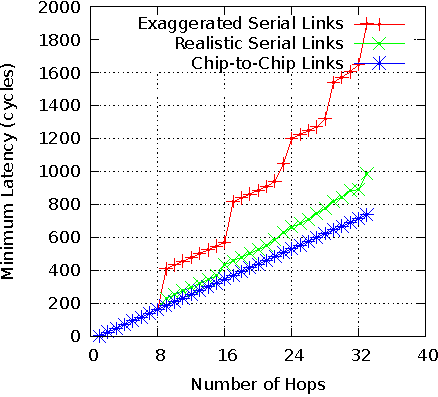
\includegraphics[width=\textwidth]{figures/min-time-for-hops}
						\caption{Minimum latencies.}
						\label{fig:min-time-for-hops}
					\end{subfigure}
					\begin{subfigure}[t]{0.45\textwidth}
						\centering
						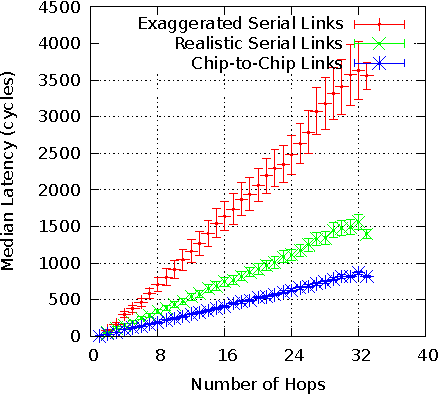
\includegraphics[width=\textwidth]{figures/median-time-for-hops-with-errbars}
						\caption{Median latencies, error bars $=
						0.1\times\textrm{Inter-Quartile Range}$.}
						\label{fig:median-time-for-hops-with-errbars}
					\end{subfigure}
					
					
					\caption{Packet latencies for various types of board-to-board
					links.}
					\label{fig:time-for-hops}
				\end{figure}
				
				Steps can be seen every time the number of hops passes a multiple of 8,
				the number of consecutive chips in any single dimension on a board,
				after which a board-to-board link is crossed causing increased latency.
				This step change can be seen clearly in the exaggerated links but is
				also visible in realistic links.
				
				An extra step appears at 28 hops, the cause of which is not currently
				known by the author.
				
				The median latency of an $n$-hop path increases smoothly as shown in
				figure \ref{fig:median-time-for-hops-with-errbars} as the probability of
				crossing a boundary increases with the number of hops carried out. From
				the gradient of these lines it can be seen that the realistic serial links
				result in an 80.4\% latency overhead.
			
			\subsubsection{Na\"ive Routing Effects}
				
				The routing scheme used by current SpiNNaker simulations is based on
				dimension order routing. This scheme assumes that all `hops' take the
				same amount of time in order to generate routes with minimal-latency.
				This assumption breaks down in heterogeneous systems.
				
				Figure \ref{fig:packet-latency-unloaded} shows how the latencies vary
				across an idle system from a single point. It can be seen that where board
				boundaries (shown in white) are crossed there is a general increase in
				latency. Because of this, the contours are visibly distorted from the
				expected hexagonal shape. This is particularly visible at the bottom left
				and top right of the figure.
				
				\begin{figure}
					\centering
					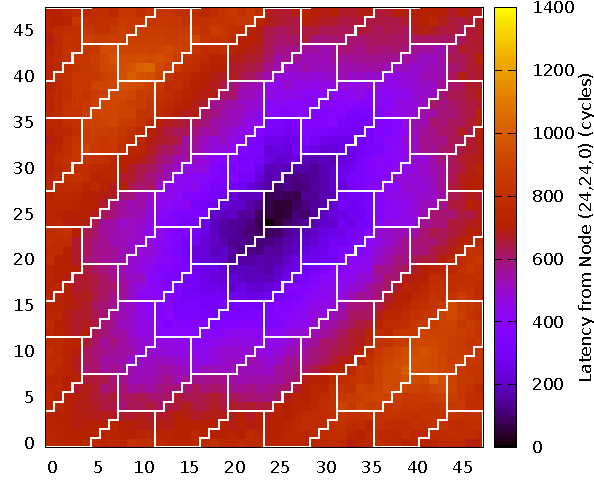
\includegraphics[width=0.7\textwidth]{figures/packet-latency-unloaded.pdf}
					
					\caption[Heat-map of average packet latency.]{Heat-map of average
					packet latency to each chip from the central chip. Note: a skewed
					perspective is used.}
					
					\label{fig:packet-latency-unloaded}
				\end{figure}
				
				A step in latency is also visible within individual boards as can be
				seen in figure \ref{fig:packet-latency-closeup-exaggerated}. Here there
				are clear edges where dimension order routing traverses the dimensions
				in an order which incurs an extra board crossing. This effect is visible
				as a step-change in latency along the diagonals of the upper-right
				boards.
		
				\begin{figure}
					\center
					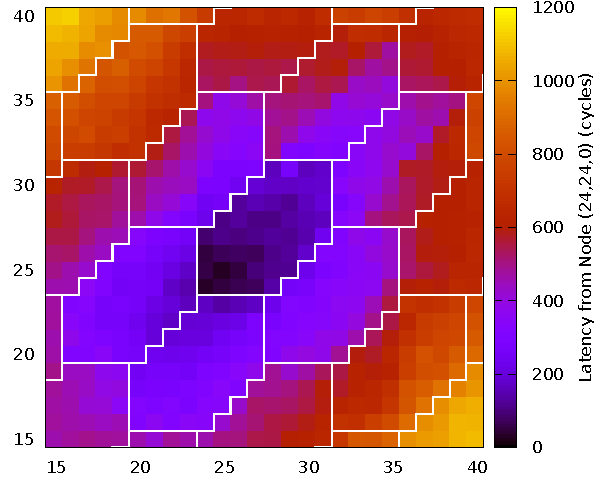
\includegraphics[width=0.7\textwidth]{figures/packet-latency-closeup-exaggerated.pdf}
					
					\caption[Latency to a subset of chips with exaggerated board-to-board
					latency.]{Latency to each chip from the central chip (24,24) to a
					section of a $48\times{}48$ system. The serial latency in this system
					has been exaggerated to aid visibility but the effect is still present
					with realistic latencies.}
					
					\label{fig:packet-latency-closeup-exaggerated}
				\end{figure}
		
		\subsection{Conclusions}
			
			Though at first sight the 80.4\% latency penalty seems severe, for
			SpiNNaker's target of SNNs running at 1 ms time steps this is not fatal.
			The new median latency is still only around 7.5 $\mu$s for the longest
			possible path, very much smaller than 1 ms deadline.  For much the same
			reason, the effects of na\"ively routing packets should also not affect
			current simulation schemes significantly.
			
			For other more latency sensitive applications such as finer-grained neural
			simulations, the increase in latency due to poor routing choices may still
			be problematic.
			
			It is worth noting that the simulations carried out were limited in size,
			duration and traffic complexity by the performance of the simulator. An
			improved simulator would allow larger models to be simulated using more
			realistic networks. One possible approach is to extend the simulator used
			by Navaridas et al. and this is discussed in
			\S\ref{sec:simulator-improvement-plan}.
		
	
	\section{Wiring-Up Large SpiNNaker Machines}
		
		\label{sec:wiring-up-large-spinnaker-machines}
		
		One of the practical constraints on the topologies is the use of wires to
		connect parts of the system together.  Chief amongst these concerns are the
		following:
		
		\begin{description}
			
			\item[Wire Cost] The choice of cabling used has a direct impact on the
			financial cost of the wiring. Higher quality materials or increased
			numbers of wires can substantially drive up the cost of the cable and
			connectors required.
			
			\item[Wire Length] Long wires have higher capacitances than short ones
			limiting the rate at which data can be transmitted.
			
			\item[Wiring Complexity] Ultimately the system will need to be assembled
			(usually) by hand so keeping wiring patterns simple is important to
			prevent wiring mistakes.
			
		\end{description}
		
		The SpiNNaker interconnect topology was studied to confirm the existence of
		a practical wiring scheme which satisfies all of the above properties. The
		principles of the machine's construction suggested by Davidson
		\cite{davidsonWiring} and Furber \cite{furber13email} were used as the basis
		for a tool used to model and experiment with possible configurations. This
		section explains the mapping developed and how it meets the above
		requirements. Finally, the section concludes with a description of the tool
		and the future work which remains.
		
		\subsection{Reducing Wiring Length}
			
			\label{sec:folding-toroids}
			
			In figure \ref{fig:boardsLogical}, touching boards are connected and the
			lines represent wires which complete the toroid by connecting opposing
			edges. While the majority of wires are very short (they connect two boards
			which are side-by-side), some wires must cross the entire system's length.
			To remove long wires from a toroid network, the network can be folded
			\cite{dally04}. An example of this process is shown for a simple
			ring-network (a 1-dimensional toroid) in figure \ref{fig:folding}.
			
			\begin{figure}
				\center
				\input{|"python figures/boardsLogical.py"}
				\caption[Logical arrangement of boards in a $4\times4$ threeboard
				SpiNNaker system.]{Logical arrangement of boards in a $4\times4$
				threeboard SpiNNaker system. Touching boards are connected. Coloured
				lines represent long connections travelling {\color{red}North/South},
				{\color{green}North-East/South-West} and {\color{blue}East/West}.}
				\label{fig:boardsLogical}
			\end{figure}
			
			\begin{figure}
				\begin{subfigure}[b]{\textwidth}
					\center
					\begin{tikzpicture}[thick,inner sep=0.1cm]
	\node [fill,circle] (node 153942796) at (0.000000,0.000000) {};
	\node [fill,circle] (node 160312652) at (1.000000,0.000000) {};
	\node [fill,circle] (node 160312684) at (2.000000,0.000000) {};
	\node [fill,circle] (node 160312716) at (3.000000,0.000000) {};
	\node [fill,circle] (node 160312812) at (4.000000,0.000000) {};
	\node [fill,circle] (node 160312908) at (5.000000,0.000000) {};
	\node [fill,circle] (node 160313036) at (6.000000,0.000000) {};
	\node [fill,circle] (node 160313164) at (7.000000,0.000000) {};
	\node [fill,circle] (node 160313292) at (8.000000,0.000000) {};
	\node [fill,circle] (node 160444524) at (9.000000,0.000000) {};
	\node [fill,circle] (node 160444652) at (10.000000,0.000000) {};
	\node [fill,circle] (node 160444812) at (11.000000,0.000000) {};
	
	\draw (node 153942796)
							         .. controls +(-1.000000,0.500000)
							                 and +(1.000000,0.500000)
							         .. (node 160444812);
	\draw (node 153942796) -- (node 160312652);
	\draw (node 160312652) -- (node 160312684);
	\draw (node 160312684) -- (node 160312716);
	\draw (node 160312716) -- (node 160312812);
	\draw (node 160312812) -- (node 160312908);
	\draw (node 160312908) -- (node 160313036);
	\draw (node 160313036) -- (node 160313164);
	\draw (node 160313164) -- (node 160313292);
	\draw (node 160313292) -- (node 160444524);
	\draw (node 160444524) -- (node 160444652);
	\draw (node 160444652) -- (node 160444812);
\end{tikzpicture}

					\caption{A ring network}
					\label{fig:ringLong}
				\end{subfigure}
				
				\vspace{2ex}
				
				\begin{subfigure}[b]{\textwidth}
					\center
					\begin{tikzpicture}[thick,inner sep=0.1cm]
	\node [fill,circle] (node 151878444) at (0.000000,0.000000) {};
	\node [fill,circle] (node 158252396) at (2.000000,0.000000) {};
	\node [fill,circle] (node 158252428) at (4.000000,0.000000) {};
	\node [fill,circle] (node 158252460) at (6.000000,0.000000) {};
	\node [fill,circle] (node 158252556) at (8.000000,0.000000) {};
	\node [fill,circle] (node 158252652) at (10.000000,0.000000) {};
	\node [fill,circle] (node 158252780) at (11.000000,0.500000) {};
	\node [fill,circle] (node 158252908) at (9.000000,0.500000) {};
	\node [fill,circle] (node 158253036) at (7.000000,0.500000) {};
	\node [fill,circle] (node 158384268) at (5.000000,0.500000) {};
	\node [fill,circle] (node 158384396) at (3.000000,0.500000) {};
	\node [fill,circle] (node 158384556) at (1.000000,0.500000) {};
	
	\draw (node 151878444) -- (node 158384556);
	\draw (node 151878444) -- (node 158252396);
	\draw (node 158252396) -- (node 158252428);
	\draw (node 158252428) -- (node 158252460);
	\draw (node 158252460) -- (node 158252556);
	\draw (node 158252556) -- (node 158252652);
	\draw (node 158252652) -- (node 158252780);
	\draw (node 158252780) -- (node 158252908);
	\draw (node 158252908) -- (node 158253036);
	\draw (node 158253036) -- (node 158384268);
	\draw (node 158384268) -- (node 158384396);
	\draw (node 158384396) -- (node 158384556);
\end{tikzpicture}

					\caption{Folded in half}
					\label{fig:ringFolded}
				\end{subfigure}
				
				\vspace{2ex}
				
				\begin{subfigure}[b]{\textwidth}
					\center
					\begin{tikzpicture}[thick,inner sep=0.1cm]
	\node [fill,circle] (node 155478860) at (0.000000,0.000000) {};
	\node [fill,circle] (node 161861004) at (2.000000,0.000000) {};
	\node [fill,circle] (node 161861036) at (4.000000,0.000000) {};
	\node [fill,circle] (node 161861068) at (6.000000,0.000000) {};
	\node [fill,circle] (node 161861164) at (8.000000,0.000000) {};
	\node [fill,circle] (node 161861260) at (10.000000,0.000000) {};
	\node [fill,circle] (node 161861388) at (11.000000,0.000000) {};
	\node [fill,circle] (node 161861516) at (9.000000,0.000000) {};
	\node [fill,circle] (node 161988652) at (7.000000,0.000000) {};
	\node [fill,circle] (node 161988780) at (5.000000,0.000000) {};
	\node [fill,circle] (node 161988908) at (3.000000,0.000000) {};
	\node [fill,circle] (node 161989068) at (1.000000,0.000000) {};
	
	\draw (node 155478860) -- (node 161989068);
	\draw (node 155478860)
							         .. controls +(1.000000,0.500000)
							                 and +(-1.000000,0.500000)
							         .. (node 161861004);
	\draw (node 161861004)
							         .. controls +(1.000000,0.500000)
							                 and +(-1.000000,0.500000)
							         .. (node 161861036);
	\draw (node 161861036)
							         .. controls +(1.000000,0.500000)
							                 and +(-1.000000,0.500000)
							         .. (node 161861068);
	\draw (node 161861068)
							         .. controls +(1.000000,0.500000)
							                 and +(-1.000000,0.500000)
							         .. (node 161861164);
	\draw (node 161861164)
							         .. controls +(1.000000,0.500000)
							                 and +(-1.000000,0.500000)
							         .. (node 161861260);
	\draw (node 161861260) -- (node 161861388);
	\draw (node 161861388)
							         .. controls +(-1.000000,0.500000)
							                 and +(1.000000,0.500000)
							         .. (node 161861516);
	\draw (node 161861516)
							         .. controls +(-1.000000,0.500000)
							                 and +(1.000000,0.500000)
							         .. (node 161988652);
	\draw (node 161988652)
							         .. controls +(-1.000000,0.500000)
							                 and +(1.000000,0.500000)
							         .. (node 161988780);
	\draw (node 161988780)
							         .. controls +(-1.000000,0.500000)
							                 and +(1.000000,0.500000)
							         .. (node 161988908);
	\draw (node 161988908)
							         .. controls +(-1.000000,0.500000)
							                 and +(1.000000,0.500000)
							         .. (node 161989068);
\end{tikzpicture}

					\caption{Interleaved}
					\label{fig:ringInterleaved}
				\end{subfigure}
				
				\caption[Folding a ring network.]{The process of folding a ring network
				to reduce the maximum wire length.}
				\label{fig:folding}
			\end{figure}
			
			\begin{figure}
				\center
				\begin{subfigure}[b]{\textwidth}
					\center
					\input{|"python figures/boardsFoldedShift.py"}
					\caption{Shift boards on the left to the right to form a rectangle.}
					\label{fig:boardsFoldedShift}
				\end{subfigure}
				
				\vspace{2ex}
				
				\begin{subfigure}[b]{\textwidth}
					\center
					\input{|"python figures/boardsFoldedSpaced.py"}
					\caption{Fold along the gaps in this figure. (Wires omitted for
					clarity.)}
					\label{fig:boardsFoldedSpaced}
				\end{subfigure}
				
				\vspace{2ex}
				
				\begin{subfigure}[b]{\textwidth}
					\center
					\input{|"python figures/boardsFoldedInterleaved.py"}
					\caption{The (more complex) wiring after folding. (Shown here with
					squares as hexagons do not visually fit together after folding and
					interleaving.)}
					\label{fig:boardsFoldedInterleaved}
				\end{subfigure}
				
				\caption[Folding SpiNNaker.]{The process of folding SpiNNaker. Coloured
				lines represent wires travelling {\color{red}North/South},
				{\color{green}North-East/South-West} and {\color{blue}East/West}.}
				\label{fig:boardsFolded}
			\end{figure}
			
			This process is generalised to SpiNNaker's boards as shown in figure
			\ref{fig:boardsFolded}. The first step (figure
			\ref{fig:boardsFoldedShift}) transforms the rhombus-like arrangement of
			boards into a rectangle which is more easily folded.
			
			In the next step, the design is folded into four parts on the X-axis and
			into two on the Y-axis (figure \ref{fig:boardsFoldedSpaced}). It is
			necessary to fold the X-axis into four as the long, diagonal wires do not
			cross the entire system on the X-axis and instead reach half way. Folding
			in two would not bring these points any closer while folding into four
			brings them next to each other. For example, the wire travelling from the
			bottom left board to the top-middle board after folding in two would now
			have to cross from one end of the system to the other, an even longer
			distance than it had to before. As a result, the maximum wire length is
			reduced which can be seen in figure \ref{fig:boardsFoldedInterleaved}.
			While the wiring in this image appears more complex, if only one direction
			(colour) is considered at once, a certain amount of regularity can be
			seen.
			
			\label{sec:mapping-spinnaker-to-cabinets}
			
			The final step in the process is to map the boards into their real-world
			physical positions. The largest SpiNNaker system will be installed into a
			series of cabinets, each containing a number of racks (shelves) into which
			the boards are slotted and wired up. Figure \ref{fig:spinnaker106} shows a
			possible rack placement scheme for the largest planned SpiNNaker system of
			$20\times20$ threeboards.
			
			\begin{figure}
				\center
				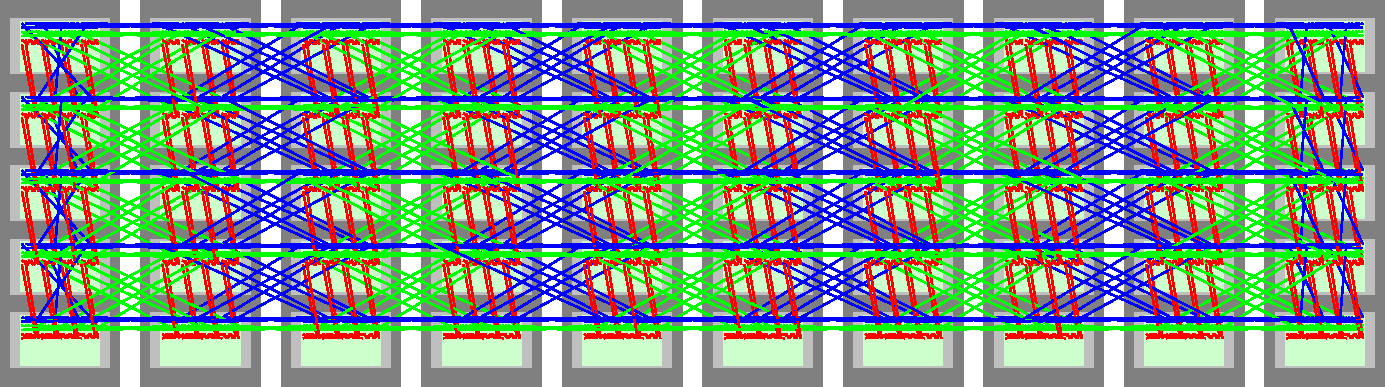
\includegraphics[width=\textwidth]{figures/spinnaker106}
				\caption[SpiNNaker machine mapped into cabinets and racks.]{The largest
				SpiNNaker machine with 1,200 boards ($20\times20$ threeboards) and
				1,036,800 cores mapped into 10 cabinets of 5 racks each.  Coloured lines
				represent wires connecting {\color{red}North/South},
				{\color{green}North-East/South-West} and {\color{blue}East/West} links.}
				\label{fig:spinnaker106}
			\end{figure}
			
			Even though the system is physically several metres long, the longest wire
			will only be around one metre in length which is within the tolerances of
			the high-speed link technology. This placement scheme, therefore, meets
			the wire-length requirement, and due to the use of high-speed serial links
			using commodity cables as described earlier, the wire-cost requirement.
			
		\subsection{Wiring Complexity}
			
			The final concern is that it should not be too complex to
			be installed by hand. The large-scale SpiNNaker machine will contain 3,600
			cables and so it is clearly not practical to have to look up each
			individual connection before wiring it up. Though it is clear that the
			folded arrangement is substantially less regular than the original layout,
			some regularity remains.
			
			By splitting up the wiring tasks by the logical direction (and thus by the
			connector on the board) it is clear that a large amount of regularity
			exists in each group of cables (consider each colour separately in figure
			\ref{fig:spinnaker106}). If the task is further split depending on whether
			the cables stay within a rack or cabinet, batches of identical racks and
			cabinets can be wired up independently before being linked together later.
			For example, the cables connecting North to South (shown in red) remain
			entirely within a cabinet meaning all North/South wiring can be completed
			independently for each cabinet.
			
			Based on the above observations, the connections for all 3,600 cables can
			be described using only 53 instructions rather than 3,200. This satisfies
			the final constraint on wiring complexity.
		
		\subsection{`SpiNNer' Wiring Guide Generator}
			
			As part of this work SpiNNer, a wiring modelling library and wiring guide
			generator, was produced to assist in the construction of SpiNNaker systems
			built from multiple boards. These tools help avoid the error prone process
			of manually visualising the various transformations required during the
			mapping of boards to racks.
			
			The modelling library allows transformations, such as folding, to be
			easily applied to a network of boards. From the transformed network,
			various measurements such as the maximum physical wire length can then be
			directly determined. Using this library the largest SpiNNaker machine can
			be described in 10 lines of code.
			
			The wiring guide generator produces illustrated documents using \LaTeX{}
			which describe the wiring for arbitrarily sized machines\footnote{Many of
			the figures in this section were adapted from wiring guides generated by
			SpiNNer.}. Metrics such as the distribution of wire lengths are included
			along with instructions for wiring the system up. At the time of writing,
			the largest prototype system constructed, a single threeboard, has been
			successfully assembled in a manner consistent with the generated wiring
			guide.
		
		\subsection{Further Work}
			
			The wiring guide generator is currently only capable of producing
			exhaustive wiring descriptions with one instruction for each of the 3,600
			cables. The foundations for extracting regularity currently exist in
			experimental form and must eventually be integrated into the wiring guide
			generator.
			
			In addition, further work may be carried out to test alternative wiring
			schemes. In the current scheme, a large proportion of the cables cross
			between different cabinets. As a result a significant amount of the wiring
			cannot be done in isolated batches. An alternative scheme may be able to
			reduce this number and further simplify the task of wiring.
	
	\section{Small-World Super-Computers}
		
		\label{sec:small-world-super-computers}
		
		Small-world networks are graphs with a very large number of nodes but,
		within which, the maximum shortest-path length is very small, despite each
		node having a relatively small number of edges. They also contain `clusters'
		of well connected nodes, in contrast with random graphs (which may also
		fulfil the first criterion).
		
		This type of network is often found in nature, perhaps most famously in
		social networks. This property was first observed in 1929 by Hungarian
		author Frigyes Karinthy\cite{karinthy29} and has become popularly known as
		the theory of `six degrees of separation'. This theory states that for any
		two people, chosen at random, there is a chain of at most 6 acquaintances
		which connects them.
		
		This property of maintaining low maximum shortest-path length while still
		remaining locally well connected is desirable for certain computational
		problems. In neural simulations most communication is local but with some
		longer connections existing. The clustering property of small world networks
		means these local connections can be well catered for while the low maximum
		shortest-path length means longer connections are still quick for very large
		models.
		
		\subsection{Network Construction}
		
			Watts and Strogatz have proposed an algorithm for randomly constructing
			networks with small-world properties \cite{watts98}. The algorithm begins
			by creating a ring network with each node connecting to a fixed number of
			its neighbours (figure \ref{fig:ringNetworkB0}). In the next step, with a
			probability of $\beta$, each edge may be replaced by a random connection.
			For $0 < \beta < 1$, the networks produced exhibit varying degrees of the
			small-world properties (figure \ref{fig:ringNetworkB02}).  Finally, in the
			extreme case where $\beta=1$, the network devolves into a random network
			(figure \ref{fig:ringNetworkB1}).
			
			\begin{figure}
				\center
				\begin{subfigure}[t]{0.3\textwidth}
					\center
					\begin{tikzpicture}[thick,inner sep=0.1cm]
	\foreach \t in {30,60,...,360}{
		\node [fill,circle] at (\t:2) {};
		\draw (\t:2) -- (\t+30:2);
		\draw (\t:2) -- (\t+60:2);
	}
\end{tikzpicture}


					\caption{Ring ($\beta = 0.0$)}
					\label{fig:ringNetworkB0}
				\end{subfigure}
				\begin{subfigure}[t]{0.3\textwidth}
					\center
					\newcommand{\mayberandompath}[2]{
	\pgfmathsetmacro{\choice}{random(5)}
	\pgfmathsetmacro{\myrand}{random(12)*30}
	\ifthenelse{\equal{\choice}{1.0}}{
		\draw (#1:2) -- (#2+\myrand:2);
	}{
		\draw (#1:2) -- (#2:2);
	}
}

\begin{tikzpicture}[thick,inner sep=0.1cm]
	\foreach \t in {30,60,...,360}{
		\node [fill,circle] at (\t:2) {};
		\mayberandompath{\t}{\t+30}
		\mayberandompath{\t}{\t+60}
	}
\end{tikzpicture}

					\caption{Watts-Strogatz ($\beta = 0.2$)}
					\label{fig:ringNetworkB02}
				\end{subfigure}
				\begin{subfigure}[t]{0.3\textwidth}
					\center
					\newcommand{\mayberandompath}[2]{
	\pgfmathsetmacro{\myrand}{random(12)*30}
	\draw (#1:2) -- (#2+\myrand:2);
}

\begin{tikzpicture}[thick,inner sep=0.1cm]
	\foreach \t in {30,60,...,360}{
		\node [fill,circle] at (\t:2) {};
		\mayberandompath{\t}{\t+30}
		\mayberandompath{\t}{\t+60}
	}
	
\end{tikzpicture}

					\caption{Random ($\beta = 1.0$)}
					\label{fig:ringNetworkB1}
				\end{subfigure}
				
				\caption{Watts-Strogatz networks with a range of rewiring
				probabilities.}
				\label{fig:ringNetwork}
			\end{figure}
			
			This algorithm is readily extended to torus topologies. In this work, a
			$k$-ary 2-cube (a two dimensional torus $k$ nodes long in each dimension)
			was used as the initial network as in figure \ref{fig:torusNetworkB0}.
			Random permutations are introduced as in the Watts-Strogatz model
			resulting in a network such as figure \ref{fig:torusNetworkB01}.
			
			\begin{figure}
				\center
				\begin{subfigure}[t]{0.45\textwidth}
					\center
					\begin{tikzpicture}[thick,inner sep=0.1cm]
	\clip (-0.5,-0.5) rectangle (5.5,5.5);
	
	\node [fill,circle] (node 146024940) at (0,0) {};
	\node [fill,circle] (node 152407084) at (1,0) {};
	\node [fill,circle] (node 152406988) at (2,0) {};
	\node [fill,circle] (node 152407180) at (3,0) {};
	\node [fill,circle] (node 152407276) at (4,0) {};
	\node [fill,circle] (node 152407404) at (5,0) {};
	\node [fill,circle] (node 152407564) at (0,1) {};
	\node [fill,circle] (node 152407692) at (1,1) {};
	\node [fill,circle] (node 152407724) at (2,1) {};
	\node [fill,circle] (node 152407788) at (3,1) {};
	\node [fill,circle] (node 152407820) at (4,1) {};
	\node [fill,circle] (node 152407948) at (5,1) {};
	\node [fill,circle] (node 152531052) at (0,2) {};
	\node [fill,circle] (node 152531148) at (1,2) {};
	\node [fill,circle] (node 152531180) at (2,2) {};
	\node [fill,circle] (node 152531212) at (3,2) {};
	\node [fill,circle] (node 152531276) at (4,2) {};
	\node [fill,circle] (node 152537548) at (5,2) {};
	\node [fill,circle] (node 152553292) at (0,3) {};
	\node [fill,circle] (node 152553836) at (1,3) {};
	\node [fill,circle] (node 152554092) at (2,3) {};
	\node [fill,circle] (node 152554668) at (3,3) {};
	\node [fill,circle] (node 152554892) at (4,3) {};
	\node [fill,circle] (node 152580172) at (5,3) {};
	\node [fill,circle] (node 152580940) at (0,4) {};
	\node [fill,circle] (node 152581804) at (1,4) {};
	\node [fill,circle] (node 152610924) at (2,4) {};
	\node [fill,circle] (node 152609420) at (3,4) {};
	\node [fill,circle] (node 152656748) at (4,4) {};
	\node [fill,circle] (node 152656844) at (5,4) {};
	\node [fill,circle] (node 152656972) at (0,5) {};
	\node [fill,circle] (node 152657068) at (1,5) {};
	\node [fill,circle] (node 152657100) at (2,5) {};
	\node [fill,circle] (node 152657132) at (3,5) {};
	\node [fill,circle] (node 152657164) at (4,5) {};
	\node [fill,circle] (node 152657260) at (5,5) {};
	
	\draw (node 146024940)
							         .. controls +(0.500000,-1.000000)
							                 and +(0.500000,1.000000)
							         .. (node 152656972);
	\draw (node 146024940)
							         .. controls +(-1.000000,0.500000)
							                 and +(1.000000,0.500000)
							         .. (node 152407404);
	\draw (node 146024940) -- (node 152407084);
	\draw (node 146024940) -- (node 152407564);
	\draw (node 152407084) -- (node 152407692);
	\draw (node 152407084)
							         .. controls +(0.500000,-1.000000)
							                 and +(0.500000,1.000000)
							         .. (node 152657068);
	\draw (node 152406988) -- (node 152407180);
	\draw (node 152406988) -- (node 152407724);
	\draw (node 152406988) -- (node 152407084);
	\draw (node 152406988)
							         .. controls +(0.500000,-1.000000)
							                 and +(0.500000,1.000000)
							         .. (node 152657100);
	\draw (node 152407180)
							         .. controls +(0.500000,-1.000000)
							                 and +(0.500000,1.000000)
							         .. (node 152657132);
	\draw (node 152407180) -- (node 152407276);
	\draw (node 152407180) -- (node 152407788);
	\draw (node 152407276) -- (node 152407404);
	\draw (node 152407276) -- (node 152407820);
	\draw (node 152407276)
							         .. controls +(0.500000,-1.000000)
							                 and +(0.500000,1.000000)
							         .. (node 152657164);
	\draw (node 152407404) -- (node 152407948);
	\draw (node 152407404)
							         .. controls +(0.500000,-1.000000)
							                 and +(0.500000,1.000000)
							         .. (node 152657260);
	\draw (node 152407564)
							         .. controls +(-1.000000,0.500000)
							                 and +(1.000000,0.500000)
							         .. (node 152407948);
	\draw (node 152407564) -- (node 152531052);
	\draw (node 152407564) -- (node 152407692);
	\draw (node 152407692) -- (node 152407724);
	\draw (node 152407692) -- (node 152531148);
	\draw (node 152407724) -- (node 152407788);
	\draw (node 152407724) -- (node 152531180);
	\draw (node 152407788) -- (node 152407820);
	\draw (node 152407788) -- (node 152531212);
	\draw (node 152407820) -- (node 152531276);
	\draw (node 152407820) -- (node 152407948);
	\draw (node 152407948) -- (node 152537548);
	\draw (node 152531052) -- (node 152553292);
	\draw (node 152531052)
							         .. controls +(-1.000000,0.500000)
							                 and +(1.000000,0.500000)
							         .. (node 152537548);
	\draw (node 152531052) -- (node 152531148);
	\draw (node 152531148) -- (node 152553836);
	\draw (node 152531148) -- (node 152531180);
	\draw (node 152531180) -- (node 152554092);
	\draw (node 152531180) -- (node 152531212);
	\draw (node 152531212) -- (node 152531276);
	\draw (node 152531212) -- (node 152554668);
	\draw (node 152531276) -- (node 152537548);
	\draw (node 152531276) -- (node 152554892);
	\draw (node 152537548) -- (node 152580172);
	\draw (node 152553292) -- (node 152580940);
	\draw (node 152553292)
							         .. controls +(-1.000000,0.500000)
							                 and +(1.000000,0.500000)
							         .. (node 152580172);
	\draw (node 152553292) -- (node 152553836);
	\draw (node 152553836) -- (node 152554092);
	\draw (node 152553836) -- (node 152581804);
	\draw (node 152554092) -- (node 152610924);
	\draw (node 152554092) -- (node 152554668);
	\draw (node 152554668) -- (node 152554892);
	\draw (node 152554668) -- (node 152609420);
	\draw (node 152554892) -- (node 152580172);
	\draw (node 152554892) -- (node 152656748);
	\draw (node 152580172) -- (node 152656844);
	\draw (node 152580940)
							         .. controls +(-1.000000,0.500000)
							                 and +(1.000000,0.500000)
							         .. (node 152656844);
	\draw (node 152580940) -- (node 152656972);
	\draw (node 152580940) -- (node 152581804);
	\draw (node 152581804) -- (node 152610924);
	\draw (node 152581804) -- (node 152657068);
	\draw (node 152610924) -- (node 152657100);
	\draw (node 152609420) -- (node 152656748);
	\draw (node 152609420) -- (node 152610924);
	\draw (node 152609420) -- (node 152657132);
	\draw (node 152656748) -- (node 152656844);
	\draw (node 152656748) -- (node 152657164);
	\draw (node 152656844) -- (node 152657260);
	\draw (node 152656972)
							         .. controls +(-1.000000,0.500000)
							                 and +(1.000000,0.500000)
							         .. (node 152657260);
	\draw (node 152656972) -- (node 152657068);
	\draw (node 152657068) -- (node 152657100);
	\draw (node 152657100) -- (node 152657132);
	\draw (node 152657132) -- (node 152657164);
	\draw (node 152657164) -- (node 152657260);
\end{tikzpicture}

					\caption{Unmodified torus ($\beta=0.0$)}
					\label{fig:torusNetworkB0}
				\end{subfigure}
				\begin{subfigure}[t]{0.45\textwidth}
					\center
					\begin{tikzpicture}[thick,inner sep=0.1cm]
	\clip (-0.5,-0.5) rectangle (5.5,5.5);
	
	\node [fill,circle] (node 163015180) at (0,0) {};
	\node [fill,circle] (node 169393228) at (1,0) {};
	\node [fill,circle] (node 169393132) at (2,0) {};
	\node [fill,circle] (node 169393324) at (3,0) {};
	\node [fill,circle] (node 169393420) at (4,0) {};
	\node [fill,circle] (node 169393548) at (5,0) {};
	\node [fill,circle] (node 169393708) at (0,1) {};
	\node [fill,circle] (node 169393836) at (1,1) {};
	\node [fill,circle] (node 169393868) at (2,1) {};
	\node [fill,circle] (node 169393932) at (3,1) {};
	\node [fill,circle] (node 169393964) at (4,1) {};
	\node [fill,circle] (node 169394092) at (5,1) {};
	\node [fill,circle] (node 169521292) at (0,2) {};
	\node [fill,circle] (node 169521388) at (1,2) {};
	\node [fill,circle] (node 169521420) at (2,2) {};
	\node [fill,circle] (node 169521452) at (3,2) {};
	\node [fill,circle] (node 169521516) at (4,2) {};
	\node [fill,circle] (node 169527788) at (5,2) {};
	\node [fill,circle] (node 169543532) at (0,3) {};
	\node [fill,circle] (node 169544076) at (1,3) {};
	\node [fill,circle] (node 169544332) at (2,3) {};
	\node [fill,circle] (node 169544908) at (3,3) {};
	\node [fill,circle] (node 169545132) at (4,3) {};
	\node [fill,circle] (node 169574508) at (5,3) {};
	\node [fill,circle] (node 169575276) at (0,4) {};
	\node [fill,circle] (node 169576140) at (1,4) {};
	\node [fill,circle] (node 169601164) at (2,4) {};
	\node [fill,circle] (node 169599660) at (3,4) {};
	\node [fill,circle] (node 169646988) at (4,4) {};
	\node [fill,circle] (node 169647084) at (5,4) {};
	\node [fill,circle] (node 169647212) at (0,5) {};
	\node [fill,circle] (node 169647308) at (1,5) {};
	\node [fill,circle] (node 169647340) at (2,5) {};
	\node [fill,circle] (node 169647372) at (3,5) {};
	\node [fill,circle] (node 169647404) at (4,5) {};
	\node [fill,circle] (node 169647500) at (5,5) {};
	
	\draw (node 163015180) -- (node 169393228);
	\draw (node 163015180)
							         .. controls +(-1.000000,0.500000)
							                 and +(1.000000,0.500000)
							         .. (node 169393548);
	\draw (node 163015180)
							         .. controls +(0.500000,-1.000000)
							                 and +(0.500000,1.000000)
							         .. (node 169575276);
	\draw (node 163015180)
							         .. controls +(0.500000,-1.000000)
							                 and +(0.500000,1.000000)
							         .. (node 169647212);
	\draw (node 169393228) -- (node 169647500);
	\draw (node 169393228) -- (node 169393836);
	\draw (node 169393228)
							         .. controls +(0.500000,-1.000000)
							                 and +(0.500000,1.000000)
							         .. (node 169647308);
	\draw (node 169393132) -- (node 169393324);
	\draw (node 169393132) -- (node 169393228);
	\draw (node 169393132)
							         .. controls +(0.500000,-1.000000)
							                 and +(0.500000,1.000000)
							         .. (node 169647340);
	\draw (node 169393132) -- (node 169393868);
	\draw (node 169393324)
							         .. controls +(0.500000,-1.000000)
							                 and +(0.500000,1.000000)
							         .. (node 169647372);
	\draw (node 169393324) -- (node 169393420);
	\draw (node 169393324) -- (node 169393932);
	\draw (node 169393420) -- (node 169393548);
	\draw (node 169393420)
							         .. controls +(0.500000,-1.000000)
							                 and +(0.500000,1.000000)
							         .. (node 169521516);
	\draw (node 169393420) -- (node 169393964);
	\draw (node 169393548)
							         .. controls +(0.500000,-1.000000)
							                 and +(0.500000,1.000000)
							         .. (node 169647500);
	\draw (node 169393548) -- (node 169394092);
	\draw (node 169393708)
							         .. controls +(-1.000000,0.500000)
							                 and +(1.000000,0.500000)
							         .. (node 169394092);
	\draw (node 169393708) -- (node 169521292);
	\draw (node 169393708) -- (node 169393836);
	\draw (node 169393836) -- (node 169393868);
	\draw (node 169393836) -- (node 169521388);
	\draw (node 169393836) -- (node 169647340);
	\draw (node 169393868) -- (node 169393932);
	\draw (node 169393932) -- (node 169647212);
	\draw (node 169393932) -- (node 169543532);
	\draw (node 169393932) -- (node 169521452);
	\draw (node 169393932) -- (node 169521516);
	\draw (node 169393964) -- (node 169394092);
	\draw (node 169394092) -- (node 169527788);
	\draw (node 169394092)
							         .. controls +(0.500000,-1.000000)
							                 and +(0.500000,1.000000)
							         .. (node 169647500);
	\draw (node 169521292)
							         .. controls +(-1.000000,0.500000)
							                 and +(1.000000,0.500000)
							         .. (node 169527788);
	\draw (node 169521292) -- (node 169543532);
	\draw (node 169521292) -- (node 169521388);
	\draw (node 169521420) -- (node 169521452);
	\draw (node 169521420) -- (node 169544332);
	\draw (node 169521452) -- (node 169544908);
	\draw (node 169521452) -- (node 169521516);
	\draw (node 169521516) -- (node 169527788);
	\draw (node 169521516) -- (node 169647340);
	\draw (node 169521516) -- (node 169545132);
	\draw (node 169527788) -- (node 169574508);
	\draw (node 169543532) -- (node 169544076);
	\draw (node 169543532) -- (node 169575276);
	\draw (node 169544076) -- (node 169544332);
	\draw (node 169544076) -- (node 169576140);
	\draw (node 169544332) -- (node 169544908);
	\draw (node 169544332) -- (node 169601164);
	\draw (node 169544908) -- (node 169545132);
	\draw (node 169544908) -- (node 169599660);
	\draw (node 169545132) -- (node 169574508);
	\draw (node 169545132) -- (node 169646988);
	\draw (node 169574508) -- (node 169647084);
	\draw (node 169575276)
							         .. controls +(-1.000000,0.500000)
							                 and +(1.000000,0.500000)
							         .. (node 169647084);
	\draw (node 169575276) -- (node 169647212);
	\draw (node 169576140) -- (node 169601164);
	\draw (node 169576140) -- (node 169647308);
	\draw (node 169601164) -- (node 169647340);
	\draw (node 169599660) -- (node 169646988);
	\draw (node 169599660) -- (node 169601164);
	\draw (node 169599660) -- (node 169647372);
	\draw (node 169646988) -- (node 169647084);
	\draw (node 169646988) -- (node 169647404);
	\draw (node 169647212)
							         .. controls +(-1.000000,0.500000)
							                 and +(1.000000,0.500000)
							         .. (node 169647500);
	\draw (node 169647212) -- (node 169647308);
	\draw (node 169647308) -- (node 169647340);
	\draw (node 169647372) -- (node 169647404);
	
\end{tikzpicture}

					\caption{Rewired torus ($\beta=0.1$)}
					\label{fig:torusNetworkB01}
				\end{subfigure}
				
				\caption{Extension of the Watts-Strogatz model to a 6-ary 2-cube.}
				\label{fig:torusNetwork}
			\end{figure}
			
			A $k$-ary $n$-cube has an average shortest path length of $\frac{nk}{4}$.
			This is because a packet travels (on average, under uniform random
			traffic) $\frac{1}{4}$ of the way around each of the $n$, $k$-node-long
			dimensions. In this case, that means the average path length is $\frac{2
			\times 6}{4} = 3$.
			
			By contrast, for the rewired version shown, the average shortest path is
			now reduced to 2.77 hops. As in Watts-Strogatz networks, the average path
			length has been brought down while much of the local connectivity remains.
		
		
		\subsection{Experiments}
			
			Experiments using a simple graph model were carried out to determine the
			effects of rewiring on shortest-path length. Figure
			\ref{fig:smallWorldTorus} shows that the shortest-path length drops
			rapidly but, as more links are rewired, returns quickly diminish. As a
			result, it can be concluded that the amount of rewiring required to
			produce a significant impact on the shortest-path length can be very
			small. These results are similar to the findings of others such as Shin et
			al. who found an increase in bandwidth (but did not test latency) when
			using small-world networks \cite{shin11}.
			
			\begin{figure}
				\center
				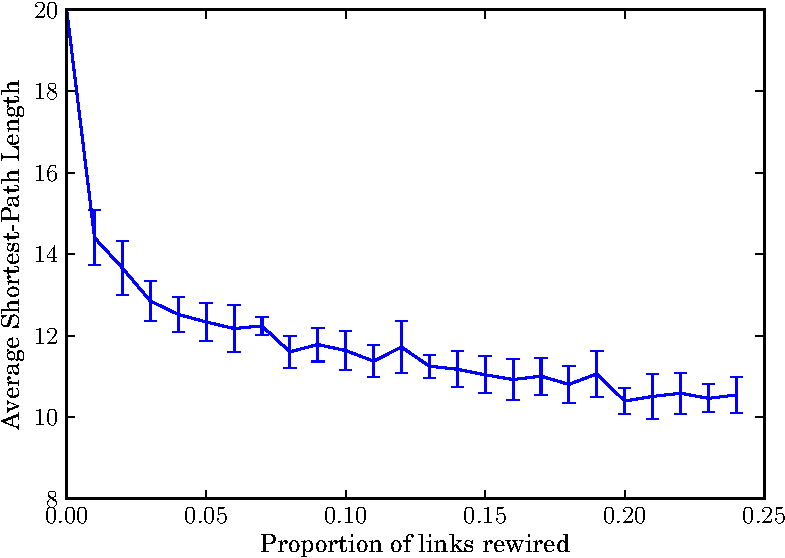
\includegraphics[width=0.7\textwidth]{figures/smallWorldTorus}
				\caption[Average shortest-path length for folded 40-ary 2-cube.]{Average
				shortest-path length for folded 40-ary 2-cube (mean of 10 runs, error
				bars show 1 standard deviation).}
				\label{fig:smallWorldTorus}
			\end{figure}
			
			Unfortunately, random wiring can be problematic for real-world systems.
			As discussed in \S\ref{sec:wiring-up-large-spinnaker-machines}, long wires
			must be avoided for many interconnection technologies and adding random
			wiring can cause many such links to be created. For example, in figure
			\ref{fig:torusNetworkB01} a long wire from the top right node stretches
			almost to the bottom left node.
			
			Work by others such as Koibuchi et al. have attempted to solve this
			problem in completely random topologies \cite{koibuchi13}.  Unfortunately
			their approaches are not applicable to networks which already feature a
			high degree of structure such as the underlying torus network used in
			these experiments. As a result, a new scheme was devised.
			
			To work around this problem, we first fold the network (as discussed
			previously in \S\ref{sec:folding-toroids}) to eliminate the long
			wrap-around wires which connect up the torus (figure
			\ref{fig:torusNetworkFB0}). Next, rewiring is carried out but with a limit
			on the maximum wire length which can be created (figure
			\ref{fig:torusNetworkFB01}).  This rewiring constrains the maximum wire to
			be 3 units long (where a unit is the spacing between each node in a given
			dimension). Even with this limitation on wire length, the maximum path
			length still drops, this time to 2.73 (from 3 in the unwired network), but
			now there are no physically long wires.
			
			\begin{figure}
				\center
				\begin{subfigure}[t]{0.45\textwidth}
					\center
					\begin{tikzpicture}[thick,inner sep=0.1cm]
	\node [fill,circle] (node 172968780) at (0.000000,0.000000) {};
	\node [fill,circle] (node 179346828) at (2.000000,0.000000) {};
	\node [fill,circle] (node 179346732) at (4.000000,0.000000) {};
	\node [fill,circle] (node 179346924) at (5.000000,0.000000) {};
	\node [fill,circle] (node 179347020) at (3.000000,0.000000) {};
	\node [fill,circle] (node 179347148) at (1.000000,0.000000) {};
	\node [fill,circle] (node 179347308) at (0.000000,2.000000) {};
	\node [fill,circle] (node 179347436) at (2.000000,2.000000) {};
	\node [fill,circle] (node 179478572) at (4.000000,2.000000) {};
	\node [fill,circle] (node 179478636) at (5.000000,2.000000) {};
	\node [fill,circle] (node 179478668) at (3.000000,2.000000) {};
	\node [fill,circle] (node 179478796) at (1.000000,2.000000) {};
	\node [fill,circle] (node 179478988) at (0.000000,4.000000) {};
	\node [fill,circle] (node 179479084) at (2.000000,4.000000) {};
	\node [fill,circle] (node 179479116) at (4.000000,4.000000) {};
	\node [fill,circle] (node 179479148) at (5.000000,4.000000) {};
	\node [fill,circle] (node 179479212) at (3.000000,4.000000) {};
	\node [fill,circle] (node 179485484) at (1.000000,4.000000) {};
	\node [fill,circle] (node 179501228) at (0.000000,5.000000) {};
	\node [fill,circle] (node 179501772) at (2.000000,5.000000) {};
	\node [fill,circle] (node 179502028) at (4.000000,5.000000) {};
	\node [fill,circle] (node 179502604) at (5.000000,5.000000) {};
	\node [fill,circle] (node 179502828) at (3.000000,5.000000) {};
	\node [fill,circle] (node 179524012) at (1.000000,5.000000) {};
	\node [fill,circle] (node 179524780) at (0.000000,3.000000) {};
	\node [fill,circle] (node 179525644) at (2.000000,3.000000) {};
	\node [fill,circle] (node 179554764) at (4.000000,3.000000) {};
	\node [fill,circle] (node 179553260) at (5.000000,3.000000) {};
	\node [fill,circle] (node 179604684) at (3.000000,3.000000) {};
	\node [fill,circle] (node 179604780) at (1.000000,3.000000) {};
	\node [fill,circle] (node 179604908) at (0.000000,1.000000) {};
	\node [fill,circle] (node 179605004) at (2.000000,1.000000) {};
	\node [fill,circle] (node 179605036) at (4.000000,1.000000) {};
	\node [fill,circle] (node 179605068) at (5.000000,1.000000) {};
	\node [fill,circle] (node 179605100) at (3.000000,1.000000) {};
	\node [fill,circle] (node 179605196) at (1.000000,1.000000) {};
	
	\draw (node 172968780) -- (node 179347148);
	\draw (node 172968780) -- (node 179604908);
	\draw (node 172968780)
							         .. controls +(1.000000,0.500000)
							                 and +(-1.000000,0.500000)
							         .. (node 179346828);
	\draw (node 172968780)
							         .. controls +(0.500000,1.000000)
							                 and +(0.500000,-1.000000)
							         .. (node 179347308);
	\draw (node 179346828)
							         .. controls +(0.500000,1.000000)
							                 and +(0.500000,-1.000000)
							         .. (node 179347436);
	\draw (node 179346828) -- (node 179605004);
	\draw (node 179346732) -- (node 179346924);
	\draw (node 179346732)
							         .. controls +(-1.000000,0.500000)
							                 and +(1.000000,0.500000)
							         .. (node 179346828);
	\draw (node 179346732) -- (node 179605036);
	\draw (node 179346732)
							         .. controls +(0.500000,1.000000)
							                 and +(0.500000,-1.000000)
							         .. (node 179478572);
	\draw (node 179346924) -- (node 179605068);
	\draw (node 179346924)
							         .. controls +(-1.000000,0.500000)
							                 and +(1.000000,0.500000)
							         .. (node 179347020);
	\draw (node 179346924)
							         .. controls +(0.500000,1.000000)
							                 and +(0.500000,-1.000000)
							         .. (node 179478636);
	\draw (node 179347020)
							         .. controls +(-1.000000,0.500000)
							                 and +(1.000000,0.500000)
							         .. (node 179347148);
	\draw (node 179347020)
							         .. controls +(0.500000,1.000000)
							                 and +(0.500000,-1.000000)
							         .. (node 179478668);
	\draw (node 179347020) -- (node 179605100);
	\draw (node 179347148) -- (node 179605196);
	\draw (node 179347148)
							         .. controls +(0.500000,1.000000)
							                 and +(0.500000,-1.000000)
							         .. (node 179478796);
	\draw (node 179347308) -- (node 179478796);
	\draw (node 179347308)
							         .. controls +(1.000000,0.500000)
							                 and +(-1.000000,0.500000)
							         .. (node 179347436);
	\draw (node 179347308)
							         .. controls +(0.500000,1.000000)
							                 and +(0.500000,-1.000000)
							         .. (node 179478988);
	\draw (node 179347436)
							         .. controls +(1.000000,0.500000)
							                 and +(-1.000000,0.500000)
							         .. (node 179478572);
	\draw (node 179347436)
							         .. controls +(0.500000,1.000000)
							                 and +(0.500000,-1.000000)
							         .. (node 179479084);
	\draw (node 179478572)
							         .. controls +(0.500000,1.000000)
							                 and +(0.500000,-1.000000)
							         .. (node 179479116);
	\draw (node 179478572) -- (node 179478636);
	\draw (node 179478636)
							         .. controls +(-1.000000,0.500000)
							                 and +(1.000000,0.500000)
							         .. (node 179478668);
	\draw (node 179478636)
							         .. controls +(0.500000,1.000000)
							                 and +(0.500000,-1.000000)
							         .. (node 179479148);
	\draw (node 179478668)
							         .. controls +(-1.000000,0.500000)
							                 and +(1.000000,0.500000)
							         .. (node 179478796);
	\draw (node 179478668)
							         .. controls +(0.500000,1.000000)
							                 and +(0.500000,-1.000000)
							         .. (node 179479212);
	\draw (node 179478796)
							         .. controls +(0.500000,1.000000)
							                 and +(0.500000,-1.000000)
							         .. (node 179485484);
	\draw (node 179478988) -- (node 179485484);
	\draw (node 179478988) -- (node 179501228);
	\draw (node 179478988)
							         .. controls +(1.000000,0.500000)
							                 and +(-1.000000,0.500000)
							         .. (node 179479084);
	\draw (node 179479084)
							         .. controls +(1.000000,0.500000)
							                 and +(-1.000000,0.500000)
							         .. (node 179479116);
	\draw (node 179479084) -- (node 179501772);
	\draw (node 179479116) -- (node 179479148);
	\draw (node 179479116) -- (node 179502028);
	\draw (node 179479148) -- (node 179502604);
	\draw (node 179479148)
							         .. controls +(-1.000000,0.500000)
							                 and +(1.000000,0.500000)
							         .. (node 179479212);
	\draw (node 179479212)
							         .. controls +(-1.000000,0.500000)
							                 and +(1.000000,0.500000)
							         .. (node 179485484);
	\draw (node 179479212) -- (node 179502828);
	\draw (node 179485484) -- (node 179524012);
	\draw (node 179501228) -- (node 179524012);
	\draw (node 179501228)
							         .. controls +(0.500000,-1.000000)
							                 and +(0.500000,1.000000)
							         .. (node 179524780);
	\draw (node 179501228)
							         .. controls +(1.000000,0.500000)
							                 and +(-1.000000,0.500000)
							         .. (node 179501772);
	\draw (node 179501772)
							         .. controls +(1.000000,0.500000)
							                 and +(-1.000000,0.500000)
							         .. (node 179502028);
	\draw (node 179501772)
							         .. controls +(0.500000,-1.000000)
							                 and +(0.500000,1.000000)
							         .. (node 179525644);
	\draw (node 179502028) -- (node 179502604);
	\draw (node 179502028)
							         .. controls +(0.500000,-1.000000)
							                 and +(0.500000,1.000000)
							         .. (node 179554764);
	\draw (node 179502604)
							         .. controls +(-1.000000,0.500000)
							                 and +(1.000000,0.500000)
							         .. (node 179502828);
	\draw (node 179502604)
							         .. controls +(0.500000,-1.000000)
							                 and +(0.500000,1.000000)
							         .. (node 179553260);
	\draw (node 179502828)
							         .. controls +(0.500000,-1.000000)
							                 and +(0.500000,1.000000)
							         .. (node 179604684);
	\draw (node 179502828)
							         .. controls +(-1.000000,0.500000)
							                 and +(1.000000,0.500000)
							         .. (node 179524012);
	\draw (node 179524012)
							         .. controls +(0.500000,-1.000000)
							                 and +(0.500000,1.000000)
							         .. (node 179604780);
	\draw (node 179524780)
							         .. controls +(0.500000,-1.000000)
							                 and +(0.500000,1.000000)
							         .. (node 179604908);
	\draw (node 179524780) -- (node 179604780);
	\draw (node 179524780)
							         .. controls +(1.000000,0.500000)
							                 and +(-1.000000,0.500000)
							         .. (node 179525644);
	\draw (node 179525644)
							         .. controls +(1.000000,0.500000)
							                 and +(-1.000000,0.500000)
							         .. (node 179554764);
	\draw (node 179525644)
							         .. controls +(0.500000,-1.000000)
							                 and +(0.500000,1.000000)
							         .. (node 179605004);
	\draw (node 179554764)
							         .. controls +(0.500000,-1.000000)
							                 and +(0.500000,1.000000)
							         .. (node 179605036);
	\draw (node 179553260)
							         .. controls +(0.500000,-1.000000)
							                 and +(0.500000,1.000000)
							         .. (node 179605068);
	\draw (node 179553260)
							         .. controls +(-1.000000,0.500000)
							                 and +(1.000000,0.500000)
							         .. (node 179604684);
	\draw (node 179553260) -- (node 179554764);
	\draw (node 179604684)
							         .. controls +(-1.000000,0.500000)
							                 and +(1.000000,0.500000)
							         .. (node 179604780);
	\draw (node 179604684)
							         .. controls +(0.500000,-1.000000)
							                 and +(0.500000,1.000000)
							         .. (node 179605100);
	\draw (node 179604780)
							         .. controls +(0.500000,-1.000000)
							                 and +(0.500000,1.000000)
							         .. (node 179605196);
	\draw (node 179604908) -- (node 179605196);
	\draw (node 179604908)
							         .. controls +(1.000000,0.500000)
							                 and +(-1.000000,0.500000)
							         .. (node 179605004);
	\draw (node 179605004)
							         .. controls +(1.000000,0.500000)
							                 and +(-1.000000,0.500000)
							         .. (node 179605036);
	\draw (node 179605036) -- (node 179605068);
	\draw (node 179605068)
							         .. controls +(-1.000000,0.500000)
							                 and +(1.000000,0.500000)
							         .. (node 179605100);
	\draw (node 179605100)
							         .. controls +(-1.000000,0.500000)
							                 and +(1.000000,0.500000)
							         .. (node 179605196);
	
\end{tikzpicture}

					\caption{Folded torus ($\beta=0.0$)}
					\label{fig:torusNetworkFB0}
				\end{subfigure}
				\begin{subfigure}[t]{0.45\textwidth}
					\center
					\begin{tikzpicture}[thick,inner sep=0.1cm]
	\node [fill,circle] (node 149404876) at (0.000000,0.000000) {};
	\node [fill,circle] (node 155782924) at (2.000000,0.000000) {};
	\node [fill,circle] (node 155782828) at (4.000000,0.000000) {};
	\node [fill,circle] (node 155783020) at (5.000000,0.000000) {};
	\node [fill,circle] (node 155783116) at (3.000000,0.000000) {};
	\node [fill,circle] (node 155910252) at (1.000000,0.000000) {};
	\node [fill,circle] (node 155910412) at (0.000000,2.000000) {};
	\node [fill,circle] (node 155910540) at (2.000000,2.000000) {};
	\node [fill,circle] (node 155910572) at (4.000000,2.000000) {};
	\node [fill,circle] (node 155910636) at (5.000000,2.000000) {};
	\node [fill,circle] (node 155910668) at (3.000000,2.000000) {};
	\node [fill,circle] (node 155910796) at (1.000000,2.000000) {};
	\node [fill,circle] (node 155910988) at (0.000000,4.000000) {};
	\node [fill,circle] (node 155911084) at (2.000000,4.000000) {};
	\node [fill,circle] (node 155911116) at (4.000000,4.000000) {};
	\node [fill,circle] (node 155911148) at (5.000000,4.000000) {};
	\node [fill,circle] (node 155911212) at (3.000000,4.000000) {};
	\node [fill,circle] (node 155921580) at (1.000000,4.000000) {};
	\node [fill,circle] (node 155937324) at (0.000000,5.000000) {};
	\node [fill,circle] (node 155937868) at (2.000000,5.000000) {};
	\node [fill,circle] (node 155938124) at (4.000000,5.000000) {};
	\node [fill,circle] (node 155938700) at (5.000000,5.000000) {};
	\node [fill,circle] (node 155959436) at (3.000000,5.000000) {};
	\node [fill,circle] (node 155960108) at (1.000000,5.000000) {};
	\node [fill,circle] (node 155960876) at (0.000000,3.000000) {};
	\node [fill,circle] (node 155961740) at (2.000000,3.000000) {};
	\node [fill,circle] (node 155990860) at (4.000000,3.000000) {};
	\node [fill,circle] (node 155989356) at (5.000000,3.000000) {};
	\node [fill,circle] (node 156040780) at (3.000000,3.000000) {};
	\node [fill,circle] (node 156040876) at (1.000000,3.000000) {};
	\node [fill,circle] (node 156041004) at (0.000000,1.000000) {};
	\node [fill,circle] (node 156041100) at (2.000000,1.000000) {};
	\node [fill,circle] (node 156041132) at (4.000000,1.000000) {};
	\node [fill,circle] (node 156041164) at (5.000000,1.000000) {};
	\node [fill,circle] (node 156041196) at (3.000000,1.000000) {};
	\node [fill,circle] (node 156074092) at (1.000000,1.000000) {};
	
	\draw (node 149404876) -- (node 155910252);
	\draw (node 149404876)
							         .. controls +(1.000000,0.500000)
							                 and +(-1.000000,0.500000)
							         .. (node 155783116);
	\draw (node 149404876)
							         .. controls +(0.500000,1.000000)
							                 and +(0.500000,-1.000000)
							         .. (node 155910412);
	\draw (node 149404876) -- (node 156041004);
	\draw (node 155782924)
							         .. controls +(0.500000,1.000000)
							                 and +(0.500000,-1.000000)
							         .. (node 155910540);
	\draw (node 155782828) -- (node 155783020);
	\draw (node 155782828)
							         .. controls +(0.500000,1.000000)
							                 and +(0.500000,-1.000000)
							         .. (node 155910572);
	\draw (node 155782828)
							         .. controls +(-1.000000,0.500000)
							                 and +(1.000000,0.500000)
							         .. (node 155782924);
	\draw (node 155782828) -- (node 156041132);
	\draw (node 155783020)
							         .. controls +(-1.000000,0.500000)
							                 and +(1.000000,0.500000)
							         .. (node 155783116);
	\draw (node 155783020)
							         .. controls +(0.500000,1.000000)
							                 and +(0.500000,-1.000000)
							         .. (node 155910636);
	\draw (node 155783020) -- (node 156041164);
	\draw (node 155783116)
							         .. controls +(-1.000000,0.500000)
							                 and +(1.000000,0.500000)
							         .. (node 155910252);
	\draw (node 155783116) -- (node 156041196);
	\draw (node 155783116)
							         .. controls +(0.500000,1.000000)
							                 and +(0.500000,-1.000000)
							         .. (node 155910668);
	\draw (node 155910252)
							         .. controls +(0.500000,1.000000)
							                 and +(0.500000,-1.000000)
							         .. (node 155910796);
	\draw (node 155910252) -- (node 156074092);
	\draw (node 155910412)
							         .. controls +(0.500000,1.000000)
							                 and +(0.500000,-1.000000)
							         .. (node 155910988);
	\draw (node 155910412)
							         .. controls +(1.000000,0.500000)
							                 and +(-1.000000,0.500000)
							         .. (node 155910540);
	\draw (node 155910540)
							         .. controls +(1.000000,0.500000)
							                 and +(-1.000000,0.500000)
							         .. (node 155910572);
	\draw (node 155910540)
							         .. controls +(0.500000,1.000000)
							                 and +(0.500000,-1.000000)
							         .. (node 155911084);
	\draw (node 155910572)
							         .. controls +(0.500000,1.000000)
							                 and +(0.500000,-1.000000)
							         .. (node 155911116);
	\draw (node 155910636) -- (node 156041132);
	\draw (node 155910636)
							         .. controls +(0.500000,1.000000)
							                 and +(0.500000,-1.000000)
							         .. (node 155938700);
	\draw (node 155910636)
							         .. controls +(0.500000,1.000000)
							                 and +(0.500000,-1.000000)
							         .. (node 155911148);
	\draw (node 155910668)
							         .. controls +(-1.000000,0.500000)
							                 and +(1.000000,0.500000)
							         .. (node 155910796);
	\draw (node 155910668)
							         .. controls +(0.500000,1.000000)
							                 and +(0.500000,-1.000000)
							         .. (node 155911212);
	\draw (node 155910796) -- (node 156040780);
	\draw (node 155910796)
							         .. controls +(0.500000,1.000000)
							                 and +(0.500000,-1.000000)
							         .. (node 155921580);
	\draw (node 155910988) -- (node 155921580);
	\draw (node 155910988)
							         .. controls +(1.000000,0.500000)
							                 and +(-1.000000,0.500000)
							         .. (node 155911084);
	\draw (node 155911084) -- (node 155990860);
	\draw (node 155911084)
							         .. controls +(1.000000,0.500000)
							                 and +(-1.000000,0.500000)
							         .. (node 155911116);
	\draw (node 155911084) -- (node 155937324);
	\draw (node 155911116) -- (node 155938124);
	\draw (node 155911116) -- (node 155911148);
	\draw (node 155911148)
							         .. controls +(-1.000000,0.500000)
							                 and +(1.000000,0.500000)
							         .. (node 155911212);
	\draw (node 155911212) -- (node 155990860);
	\draw (node 155911212) -- (node 155959436);
	\draw (node 155921580) -- (node 155960108);
	\draw (node 155937324) -- (node 155960108);
	\draw (node 155937324)
							         .. controls +(0.500000,-1.000000)
							                 and +(0.500000,1.000000)
							         .. (node 155960876);
	\draw (node 155937868)
							         .. controls +(1.000000,0.500000)
							                 and +(-1.000000,0.500000)
							         .. (node 155938124);
	\draw (node 155937868)
							         .. controls +(0.500000,-1.000000)
							                 and +(0.500000,1.000000)
							         .. (node 155961740);
	\draw (node 155937868) -- (node 156040876);
	\draw (node 155937868) -- (node 155960108);
	\draw (node 155938124)
							         .. controls +(0.500000,-1.000000)
							                 and +(0.500000,1.000000)
							         .. (node 155990860);
	\draw (node 155938124) -- (node 155938700);
	\draw (node 155938700) -- (node 155938700);
	\draw (node 155938700)
							         .. controls +(-1.000000,0.500000)
							                 and +(1.000000,0.500000)
							         .. (node 155959436);
	\draw (node 155938700)
							         .. controls +(0.500000,-1.000000)
							                 and +(0.500000,1.000000)
							         .. (node 155989356);
	\draw (node 155959436)
							         .. controls +(0.500000,-1.000000)
							                 and +(0.500000,1.000000)
							         .. (node 156040780);
	\draw (node 155959436)
							         .. controls +(-1.000000,0.500000)
							                 and +(1.000000,0.500000)
							         .. (node 155960108);
	\draw (node 155960108)
							         .. controls +(0.500000,-1.000000)
							                 and +(0.500000,1.000000)
							         .. (node 156040876);
	\draw (node 155960876) -- (node 156040876);
	\draw (node 155960876)
							         .. controls +(0.500000,-1.000000)
							                 and +(0.500000,1.000000)
							         .. (node 156041004);
	\draw (node 155960876)
							         .. controls +(1.000000,0.500000)
							                 and +(-1.000000,0.500000)
							         .. (node 155961740);
	\draw (node 155961740)
							         .. controls +(1.000000,0.500000)
							                 and +(-1.000000,0.500000)
							         .. (node 155990860);
	\draw (node 155961740)
							         .. controls +(0.500000,-1.000000)
							                 and +(0.500000,1.000000)
							         .. (node 156041100);
	\draw (node 155989356)
							         .. controls +(-1.000000,0.500000)
							                 and +(1.000000,0.500000)
							         .. (node 156040780);
	\draw (node 155989356) -- (node 155990860);
	\draw (node 155989356)
							         .. controls +(0.500000,-1.000000)
							                 and +(0.500000,1.000000)
							         .. (node 156041164);
	\draw (node 156040780)
							         .. controls +(-1.000000,0.500000)
							                 and +(1.000000,0.500000)
							         .. (node 156040876);
	\draw (node 156040780)
							         .. controls +(0.500000,-1.000000)
							                 and +(0.500000,1.000000)
							         .. (node 156041196);
	\draw (node 156040876)
							         .. controls +(0.500000,-1.000000)
							                 and +(0.500000,1.000000)
							         .. (node 156074092);
	\draw (node 156041004) -- (node 156074092);
	\draw (node 156041004)
							         .. controls +(1.000000,0.500000)
							                 and +(-1.000000,0.500000)
							         .. (node 156041100);
	\draw (node 156041100)
							         .. controls +(1.000000,0.500000)
							                 and +(-1.000000,0.500000)
							         .. (node 156041132);
	\draw (node 156041132) -- (node 156041164);
	\draw (node 156041164)
							         .. controls +(-1.000000,0.500000)
							                 and +(1.000000,0.500000)
							         .. (node 156041196);
	\draw (node 156041196)
							         .. controls +(-1.000000,0.500000)
							                 and +(1.000000,0.500000)
							         .. (node 156074092);
	
\end{tikzpicture}


					\caption{Rewired torus ($\beta=0.1$)}
					\label{fig:torusNetworkFB01}
				\end{subfigure}
				
				\caption{Rewiring a folded torus with constrained maximum wire-length.}
				\label{fig:torusNetworkF}
			\end{figure}
			
			To test the effects of limiting wire lengths when re-wiring, a parameter
			sweep was carried out for a 40-ary 2-cube. The test was carried out after
			folding once and twice in each dimension and finally when the
			network was not folded. The results are given in figure
			\ref{fig:smallWorldLimitedWiring}.
			
			\begin{figure}
				\center
				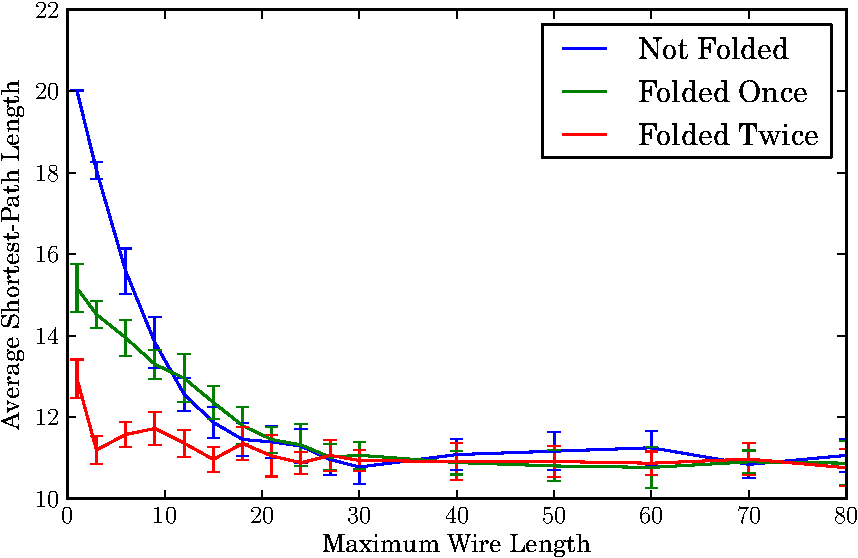
\includegraphics[width=0.7\textwidth]{figures/smallWorldLimitedWiring}
				\caption{Average shortest-path length for folded 40-ary 2-cube with 1\% rewiring}
				\label{fig:smallWorldLimitedWiring}
			\end{figure}
			
			It is clear that when wire lengths are most limited, the average
			shortest-path length improves when the network has been folded. This
			result is intuitive because after folding, physically neighbouring boards
			are no-longer logically adjacent but instead are at opposite ends of the
			system. As a result, limiting wire lengths essentially `prefers' the
			creation of logically longer links which are most likely to pull the
			average path length down.
			
			The other interesting effect is that, above a certain threshold, allowing
			longer wires has no significant effect on the average shortest-path
			length. This may be because wires which stretch further than half-way
			($\frac{k}{2}$ hops) along a given axis could be just as easily reached by
			travelling the shorter distance the other way around the axis. This
			longest useful wire length can be calculated as follows:
			\[
				\textrm{Maximum Useful Wire Length}
					= \sqrt{n \left({\frac{k}{2}}\right)^2}
					= \frac{k\sqrt{n}}{2}
			\]
			For a 40-ary 2-cube the maximum useful wire length is $20\sqrt{2} \approx
			28.3$ which can be visually confirmed in the figure.
		
		\subsection{Further Work}
			
			Figure \ref{fig:ringNetworkLimitedWires} shows valid random links in a
			small ring network with limited wire lengths. Nodes near the top and
			bottom of the ring potentially have shorter average path lengths to all
			other nodes than nodes near the left and right of the ring. This is
			because the allowed random links for top and bottom nodes connect nodes at
			greater logical distances in the ring than those allowed on the left and
			right. The result is that the average path length from two different nodes
			becomes non-uniform across nodes in different parts of the system.
			
			\begin{figure}
				\center
				\begin{tikzpicture}[thick,inner sep=0.1cm]
	\foreach [count=\n] \t in {30,60,...,360}{
		\node [fill,circle] at (90-\t:2) (node \n) {};
		\draw [help lines] (\t:2) -- (\t+30:2);
	}
	
	\draw (node 8) to (node 10);
	\draw (node 8) to (node 11);
	
	\draw (node 7) to (node 11);
	\draw (node 7) to (node 12);
	
	\draw (node 6) to (node 12);
	\draw (node 6) to (node 1);
	
	\draw (node 5) to (node 1);
	\draw (node 5) to (node 2);
	
	\draw (node 4) to (node 2);
	
\end{tikzpicture}


				\caption[Valid random links in a folded ring network with short
				wires.]{Valid random links in ring network when wires limited to a
				length of 1 unit and the network is folded as in figure
				\ref{fig:folding}.}
				\label{fig:ringNetworkLimitedWires}
			\end{figure}
			
			Further work may study the effects of this non-uniformity of average path
			length. The effects of the non-uniformity may be reduced by using greater
			degrees of folding or higher dimensional topologies. In addition, real
			systems are constrained to standard cabinets and racks, as in
			\S\ref{sec:mapping-spinnaker-to-cabinets}, which may change distribution
			of average path lengths in the system.
			
			This work could be extended to include this final mapping into more
			realistic physical placements, for example by building on the SpiNNer
			wiring modelling library. It is anticipated that the more complex
			placements resulting from higher-dimensions and realistic placement will
			result in a more uniform distribution of average path lengths.

	\chapter{Research Plan}
	
	\label{sec:research-plan}
	
	In this chapter an outline of the work to be carried out is presented. Due to
	the embryonic stage of the research, later work is presented with less detail.
	Figure \ref{fig:plan-gantt} shows a Gantt chart containing the key stages of
	the project which are outlined in chronological order in the sections below.
	
	\begin{figure}[b!]
		\center
		\begin{tikzpicture}[thick,x=0.25cm]

%%%%%%%%%%%%%%%%%%%%%%%%%%%%%%%%%%%%%%%%%%%%%%%%%%%%%%%%%%%%%%%%%%%%%%%%%%%%%%%%
% Hacked-up Gantt Library
%%%%%%%%%%%%%%%%%%%%%%%%%%%%%%%%%%%%%%%%%%%%%%%%%%%%%%%%%%%%%%%%%%%%%%%%%%%%%%%%

% An entry in the Gantt chart. Takes a label, start offset, length and slack.
% Also defines a pair of labels "[label] start" and "[label] end" which can be
% used for drawing dependency lines.
\newcommand{\ganttEntry}[4]{
	% Label
	\node (label)
				[below=1.5ex of label.south east,anchor=east,minimum height=1.7em]
				{#1}
				;
	\coordinate (gantt labels end) at (label.south east);
	
	% Box
	\draw ([shift={(#2   ,-.9ex)}]label.north east) rectangle
	      ([shift={(#2+#3,0.9ex)}]label.south east);
	
	% The tips of the box
	\coordinate (#1 end)
	         at ([shift={(#2+#3,0.9ex)}]label.south east);
	\coordinate (#1 start)
	         at ([shift={(#2   ,-.9ex)}]label.north east);
	
	% Slack line
	\draw [ultra thick]
	      ([shift={(#2+#3,0)}]$(label.north east)!0.5!(label.south east)$)
	   -- ++(#4,0);
}

\newcommand{\ganttDep}[2]{
	\draw [->,red] (#1 end) -| (#2 start);
}

\newcommand{\ganttVSep}[2]{
	\draw [#2] ([shift={(#1,0)}]gantt labels start) -- ([shift={(#1,0)}]gantt labels end);
}

% A new gantt chart. Takes a list of x-offset/label/major-label tuples. For each
% tuple a line is created with x-offset from the previous line and the span is
% labelled with "label". If major-label given, a major label will be drawn
% centered over the previous entries up until the last major-label.
\newenvironment{gantt}[1]{
	% Start the list of labels
	\node (label) [white] {Ag};
	\coordinate (gantt labels start) at (label.north east);
	\def\periods{#1}
}{
	\begin{scope}[on background layer]
		% Thick line separating from labels
		\draw (gantt labels start) -- (gantt labels end);
		
		% Start of the area covered by a "major" label
		\coordinate (gantt maj label start) at (gantt labels start);
		
		\foreach \x/\lab/\mlab in \periods {
			\coordinate (next gantt labels start) at ([shift={(\x,0)}]gantt labels start);
			\coordinate (next gantt labels end)   at ([shift={(\x,0)}]gantt labels end);
			
			% Minor label
			\node at ($(gantt labels start) !0.5! (next gantt labels start)$)
			      [anchor=west,rotate=90]
			      {\lab}
			      ;
			
			% Separator
			\ifthenelse{\equal{\mlab}{}}{
				\draw [help lines] (next gantt labels start) -- (next gantt labels end);
			}{
				\draw [help lines,thick] (next gantt labels start) -- (next gantt labels end);
			}
			
			\coordinate (gantt labels start) at (next gantt labels start);
			\coordinate (gantt labels end)   at (next gantt labels end);
			
			% Major label
			\ifthenelse{\equal{\mlab}{}}{}{
				\coordinate (next gantt maj label start) at (gantt labels start);
				\node at ($(gantt maj label start) !0.5! (next gantt maj label start)$)
				      [yshift=1cm,anchor=south]
				      {\mlab}
				      ;
				\coordinate (gantt maj label start) at (next gantt maj label start);
			}
		}
	\end{scope}
}



%%%%%%%%%%%%%%%%%%%%%%%%%%%%%%%%%%%%%%%%%%%%%%%%%%%%%%%%%%%%%%%%%%%%%%%%%%%%%%%%
% The Chart...
%%%%%%%%%%%%%%%%%%%%%%%%%%%%%%%%%%%%%%%%%%%%%%%%%%%%%%%%%%%%%%%%%%%%%%%%%%%%%%%%

\begin{gantt}{
	4/Aug/, 4/Sep/, 4/Oct/, 4/Nov/, 4/Dec/2013,%
	2/Q1/, 2/Q2/, 2/Q3/, 2/Q4/2014,%
	2/Q1/, 2/Q2/, 2/Q3/, 2/Q4/2015,%
	2/Q1/, 2/Q2/2016%
}
	\ganttEntry{SpiNNaker Modelling}          {0}{5}{3}
	\ganttEntry{Small-World SpiNNaker}        {5}{4}{1}
	\ganttEntry{Topology Comparison}          {8}{8}{4}
	\ganttEntry{Place and Routeability}       {16}{4}{0.5}
	\ganttEntry{Multicast Simulation}         {20}{1}{0.5}
	\ganttEntry{Interconnect Evaluation}      {21}{1}{0.5}
	\ganttEntry{Architecture Design}          {22}{6}{4}
	\ganttEntry{Architecture Evaluation}      {26}{4}{2}
	\ganttEntry{Thesis Writing}               {30}{8}{2}
	
	\ganttDep{SpiNNaker Modelling}{Small-World SpiNNaker};
	\ganttDep{SpiNNaker Modelling}{Topology Comparison};
	\ganttDep{SpiNNaker Modelling}{Place and Routeability};
	
	\ganttDep{Place and Routeability}{Multicast Simulation};
	
	\ganttDep{Place and Routeability}{Architecture Design};
\end{gantt}

\end{tikzpicture}

		
		\caption[Research plan Gantt chart.]{Gantt chart of proposed research plan.
		Arrows indicate dependencies, thick lines indicate slack.  Note non-linear
		scale.}
		\label{fig:plan-gantt}
	\end{figure}
	
	
	\section{SpiNNaker Modelling}
		
		% In order to experiment with the way new interconnection options affect
		% SpiNNaker an accurate model is required. Will work with Mikel and Javier to
		% extend the SpiNNaker simulator used in the original paper to include models
		% of inter-board links.
		%
		% How long will this take?
		
		As part of the ongoing SpiNNaker project a study is being carried out to
		compare how network simulations compare with the real hardware. As part of
		this work, researchers have built an FPGA accelerated model of SpiNNaker's
		interconnection network. The work hopes to verify the accuracy of the model
		against both a traditional software model and also the final silicon
		implementation. The results of this work are intended for a Journal
		publication aiming for submission around the end of September 2013.
		
		My participation in this project will be to develop the software simulation
		to model and evaluate the network implemented in SpiNNaker. Once built, this
		simulator will be valuable for my own research into alternative network
		topologies.  This section outlines in further detail the motivation and
		requirements for the simulator followed by a discussion of its applications
		for my own work.
		
		\subsection{Software Simulator Limitations}
		
			The prototype software model is built on the INSEE simulator
			\cite{navaridas11insee} which is designed to simulate a wide variety of
			networks. Unfortunately, INSEE's router model is different from that found
			in SpiNNaker and the FPGA model. The differences in their behaviour are
			outlined below.
			
			% TODO: elaborate
			
			SpiNNaker makes use of store-and-forward routing where a message must be
			fully received before it can be routed to the next point in its path. By
			contrast, INSEE is designed to support cut-through routing where once the
			first part of a message has been received it may immediately begin the
			routing process.
			
			The other key difference between INSEE and the actual SpiNNaker
			architecture is the way packets from incoming links are arbitrated. Figure
			\ref{fig:arbitration} shows the arbitration schemes for INSEE and
			SpiNNaker. INSEE uses a simple round-robin arbitration scheme while
			SpiNNaker (and the FPGA model) use a tree of arbitrators\footnote{The
			bandwidth available at each level of the arbitration tree scales with the
			maximum input bandwidth for each level.}.
			
			\begin{figure}
				\begin{subfigure}[t]{0.50\textwidth}
					\center
					\begin{tikzpicture}[thick]
	
	\node (arbitrator)
		[draw,minimum height=6cm]
		{
			\tikz[minimum height=0cm]
				\node[rotate=90]{RR};
		};
	
	\newcommand{\inputline}[2]{
		\draw [<-]
		      ($(arbitrator.north west) !#1! (arbitrator.south west)$) -- ++(-0.5,0)
		      node [left] {#2}
		      ;
	}
	\inputline{0.1}{N}
	\inputline{0.2}{S}
	\inputline{0.3}{E}
	\inputline{0.4}{W}
	\inputline{0.5}{NW}
	\inputline{0.6}{SE}
	\inputline{0.7}{P1}
	\inputline{0.8}{\ldots}
	\inputline{0.9}{P18}
	
	\draw [->]
	      ($(arbitrator.north east) !0.5! (arbitrator.south east)$) -- ++(0.5,0)
	      node [right] {Router}
	      ;
	
\end{tikzpicture}

					
					\caption{INSEE}
					\label{fig:arbitrationINSEE}
				\end{subfigure}
				\begin{subfigure}[t]{0.50\textwidth}
					\center
					\begin{tikzpicture}[thick]
	
	\newcommand{\rootarb}[3]{
		\node (#1)
			[draw,minimum height=#2] #3
			{
				\tikz[minimum height=0cm]
					\node[rotate=90]{RR};
			};
	}
	
	\newcommand{\arb}[4]{
		\rootarb{#1}{#2}{[left=0.5 of $(#4.north west) !#3! (#4.south west)$]}
		\draw [->] (#1) to (#4);
	}
	
	\rootarb{root arb}{4cm}{}
	
	\arb{nsew arb}{ 2.0cm}{0.1}{root arb}
	\arb{neswc arb}{2.0cm}{0.9}{root arb}
	
	\arb{ns arb}{  1cm}{0.1}{nsew arb}
	\arb{ew arb}{  1cm}{0.9}{nsew arb}
	\arb{nesw arb}{1cm}{0.1}{neswc arb}
	\arb{core arb}{1cm}{0.9}{neswc arb}
	
	\newcommand{\inputline}[3]{
		\draw [<-]
		      ($(#2.north west) !#1! (#2.south west)$) -- ++(-0.5,0)
		      node [left] {#3}
		      ;
	}
	\inputline{0.25}{ns arb}{N}
	\inputline{0.75}{ns arb}{S}
	
	\inputline{0.25}{ew arb}{E}
	\inputline{0.75}{ew arb}{W}
	
	\inputline{0.25}{nesw arb}{NW}
	\inputline{0.75}{nesw arb}{SE}
	
	\inputline{0.25}{core arb}{P1}
	\inputline{0.50}{core arb}{\ldots}
	\inputline{0.75}{core arb}{P18}
	
	\draw [->]
	      ($(root arb.north east) !0.5! (root arb.south east)$) -- ++(0.5,0)
	      node [right] {Router}
	      ;
	
\end{tikzpicture}

					
					\caption{SpiNNaker}
					\label{fig:arbitrationSpiNNaker}
				\end{subfigure}
				
				\caption[Incoming packet arbitration schemes in INSEE and
				SpiNNaker.]{Incoming packet arbitration schemes in INSEE and SpiNNaker.
				Boxes marked `RR' are round-robin arbitrators, P1-P18 are connections to
				local processor cores.}
				\label{fig:arbitration}
			\end{figure}
			
			This difference here extends beyond the order in which contesting requests
			will be serviced. In INSEE, each input has a buffer associated with it
			from which the router will extract messages and forward them to the input
			buffer of the next node, one per simulated cycle. In the SpiNNaker design,
			messages are buffered at each level of the tree and eventually placed in a
			pipeline within the router (equivalent to further buffering) and an output
			buffer. The interaction of all these buffers is not modelled by INSEE and
			thus the results produced are less well matched with the actual SpiNNaker
			system.
			
			% Part of the aim of the work is to produce a comparison between this
			% software model, an FPGA model and a prototype system. Successful
			% comparison of the three will allow higher certainty in results obtained
			% from other work (namely the interconnect experiments to follow).
		
		\subsection{Simulator Improvement Plan}
			
			\label{sec:simulator-improvement-plan}
			
			Given the limitations of INSEE mentioned in the previous section, two
			possible approaches must be considered. Either INSEE must be modified to
			incorporate a more realistic model of the router or an alternative
			simulator must be used.  One important factor in the decision is the
			`ramp-up' time required to gain familiarity with the INSEE code-base
			compared with the time required to develop or extend an alternative
			simulator. The other factor is the utility of the simulator for my own
			research.
			
			Since INSEE is an established tool which has been used in similar work it
			is potentially a strong choice. In order to determine its suitability for
			this work and my own research a small amount of time will be initially
			spent analysing its design. If it is found to be suitable development of
			an extended version will commence.
			
			A possible alternative to INSEE is the simulator developed during the
			preliminary interconnect study in \S\ref{sec:interconnect-modelling}.
			Like INSEE, it has been already been used to simulate the SpiNNaker
			Interconnect and so configurations exist for SpiNNaker like machines.
			Because of the author's familiarity with the tool, extending the router
			model should be straight-forward.
	
	
	\section{Small-World Network Experiments}
		
		With the extended and proven simulator developed, the next stage of my
		research will be to use it to model the behaviour of small-world style
		networks with more realistic traffic and wiring constraints.
		
		The work done in \S\ref{sec:small-world-super-computers} measured average
		shortest-path length in the networks examined. This measure corresponds to
		the average path length for uniform-random traffic in a real network with
		the same topology. In brain simulation systems such as spinnaker, much of
		the traffic is local and so uniform-random traffic is not representative.
		This work will test the performance of small-world networks with more
		realistic traffic.
		
		The other shortcoming found during the preliminary study was that when
		physical wiring was restricted in length (as in real systems), the logical
		distance covered by links in different parts of the system becomes uneven.
		Since the folding and rack/cabinet placement which takes place in real
		machines such as SpiNNaker is much more intricate than the simple torus
		studied, these effects may become insignificant.
		
		This work is intended to take around one further month including ample time
		for writing up and further experimentation with wiring schemes if required.
	
	
	\section{Topology Comparison}
		
		% Look at a whole load of popular topologies and possibly look at having
		% two/more networks.
		
		With the small-world network testing complete, the simulator should now be
		mature enough to begin further experiments with alternative, potentially
		more structured topologies. This will be done to empirically test
		alternative topologies for use in SNN simulation.
		
		This work will follow on from the experiments carried out by
		\cite{vainbrand11} which was limited to widely used, more generic network
		topologies with alternatives which may be better suited to the problem. For
		example, topologies such as express cubes \cite{dally91} offer improved
		performance for a limited amount of non-local traffic while preserving the
		local performance of mesh and torus networks.
	
	\section{Placement and Routing}
		
		Given the scale of the SpiNNaker machine and the networks it simulates, the
		NP-complete task of allocating processing tasks in each node in the system
		(placement) and routing messages between them (routing) is an important
		consideration. Current architectures, such as SpiNNaker, use table based
		routing where a lookup table is used to decide where to route messages
		arriving at each node in the system. Such systems offer a lot of flexibility
		in the routing schemes that can be implemented but also may introduce
		constraints on the complexity of routes through the system when the routing
		tables are restricted in size.
		
		The use of alternative topologies will require alternative routing schemes
		to be specified. In the above comparative work on possible topologies
		simple, na\"ive routing algorithms will be used. These simple to implement
		algorithms often result in non-optimal behaviour, especially with regard to
		load balancing\cite{dally04}. Given that systems such as SpiNNaker use
		packet-dropping flow control, where congested routes can cause packets to be
		dropped, the effects of load imbalance may cause localised areas of high
		packet losses which may significantly affect simulations.
		\cite{greenfield10}.
		
		In this phase of work alternative routing algorithms which attempt to handle
		routing table depth and congestion control will be studied. The former
		problem is similar in style to the problem faced by chip and printed circuit
		design automation tools. The latter side is covered largely by more
		conventional interconnect/network routing algorithms. Combining and
		evaluating these two approaches will be where much of this time is spent.
	
	\section{Effects of Multicast}
		
		Following on from work on basic routing, the challenge of performing routing
		for multicast traffic must be considered. Multicast routing must route a
		message from a single source to multiple destinations, in the case of
		spiking neural networks, potentially thousands of destinations.
		
		Current approaches to multicast routing again are split between chip and
		circuit design and interconnect/network routing. Chip designs often
		constrain the paths in various ways, for example to ensure that latency to
		each destination is similar. This parallels the need to try and control
		branching to minimise routing table resource. Network designs, however, are
		often designed to reduce the amount of bandwidth consumed by branching as
		late as possible. Once again, work must be done to combine and compare these
		two approaches.
	
	\section{Interconnect Technology Evaluation}
		
		% Can't use Silistix any more, HSS is nice but should we be using it
		% on-chip?
		
		Given a suitable topology, a further question is that of the actual
		implementation of the interconnect. Historically small-scale systems have
		used synchronous signals to communicate between various parts of the system.
		As systems have scaled, this is no longer feasible as clock distribution
		grows ever more difficult. Instead GALS architectures have become prominent
		where individual, synchronous components communicate via an asynchronous
		medium.
		
		The SpiNNaker chip uses an asynchronous NoC based on CHAIN
		\cite{plana07,bainbridge02} using IP from (the now defunct) Silistix Ltd.
		This interconnect is able to handle arbitration between the many incoming
		signals from on board processors and external connections to other chips.
		Since this technology is no-longer available, alternatives must be sought.
		
		SpiNNaker chips are interconnected using parallel, delay insensitive
		interconnects. These links, while adequate for the system's current scale,
		may not be trivially sped up. More suitable external interconnects will
		likely be based on high speed serial as described in
		\S\ref{sec:high-speed-serial}.
		
		Work must be done to evaluate what technologies will be best suited for us
		in a future system.
	
	\section{`SpiNNaker 2' Architecture}
		
		% It is likely that a new version of SpiNNaker will be designed with some
		% funding coming in soon. Based on the research into the interconnect here,
		% would an alternative topology be appropriate?
		
		Based on the preceding work and on further developments within in the
		SpiNNaker project, a new architecture for neural network simulation will be
		proposed. In particular the architecture is intended to be a successor to
		the SpiNNaker platform aimed at a similar communication-bound model.
		
		\subsection{Scaling}
			
			Due to the advance of Moore's law, several times more chip area will be
			available for this next generation architecture compared to the previous
			revision. It is assumed that it will be possible to fit a larger number of
			cores into a single chip along with larger memories both for the on board
			processors.
			
			The preceding work will be used to decide on the type of topology and
			routing systems to be used. It is expected that access to larger routing
			table resource as well as more area for routing logic will be available.
		
		\subsection{Interconnection Network}
			
			One of the known limitations of SpiNNaker's interconnection network is
			that it has been optimised largely for the style of traffic required while
			simulations are in progress, in particular it deals very well with small,
			multicast packets whose delivery does not need to be guaranteed, as with
			biological spikes.
			
			Other important tasks, however, are not handled as well such as
			initialisation and result collection. These tasks require reliable
			communication, typically with a relatively larger data payload. This is
			currently facilitated by the SpiNNaker Datagram Protocol (SDP)
			\cite{temple11} which allows unreliable point-to-point transmission of up
			to 64KB of data. While this offers the ability to easily load
			configurations to SpiNNaker chips, collecting data becomes more difficult.
			With the larger, multi-board systems currently in testing, contention for
			the links surrounding a central node during data-collection become
			saturated resulting in a large number of packets being dropped.
		
		\subsection{Link Technology}
			
			% Switching away from Silistix (they went bye-bye!), alternative
			% technologies, e.g. high-speed serial, might be used to link chips
			% together. Such technologies may have very different cost structures and
			% call for new network topologies. Given we currently have concentrated
			% multiplexed links, why not have the same for stuff lower down?
			
			The underlying Silistix technology used by SpiNNaker's links is not
			available for new systems and must be replaced. Based on research into
			link technologies a decision must be made for the new system. This choice
			will strongly influence the design of the network.
		
		
		\subsection{Evaluation}
			
			The proposed topology will be evaluated by simulation building on the
			simulators developed earlier in the project. It is hoped that more
			information on the actual usage and traffic patterns encountered by the
			current SpiNNaker hardware will be available to drive this simulation and
			to present a point of comparison.
		

	\chapter{Conclusion}


	
	% Number bib entries by order of appearance
	\bibliographystyle{unsrt}
	\bibliography{report}
	
\end{document}
